\documentclass{uflamon}          % classe base para a monografia

% ==============================================================================
% Utilizacao de pacotes
\usepackage[T1]{fontenc}         % usa fontes postscript com acentos
\usepackage[brazil]{babel}       % hifenização e títulos em português do Brasil
\usepackage[utf8]{inputenc}      % permite edição direta com acentos
\usepackage{amsmath}             % pacote da AMS para Matemática Avançada
\usepackage{amssymb}             % símbolos extras da AMS
\usepackage{latexsym}            % símbolos extras do LaTeX
\usepackage{graphicx}            % para inserção de gráficos
\usepackage{listings}            % para inserção de código
\usepackage{fancyvrb}            % para inserção de saídas de comandos
% \usepackage{enumerate}         % para personalizar lista enumeradas (incluso na classe)
\usepackage{longtable}           % para tabelas muito grandes NOVO!!!!

\usepackage{colortbl}            % cores em tabelas
\newcolumntype{Z}{|>{\columncolor[gray]{0.9}}l|} %cor cinza em células
% \usepackage{array}              % já incluso na classe
\newcolumntype{L}[1]{>{\raggedright\let\newline\\\arraybackslash\hspace{0pt}}m{#1}}
\newcolumntype{C}[1]{>{\centering\let\newline\\\arraybackslash\hspace{0pt}}m{#1}}
\newcolumntype{R}[1]{>{\raggedleft\let\newline\\\arraybackslash\hspace{0pt}}m{#1}}

\usepackage{multirow}            % para juntar duas linhas em uma só
\usepackage{multicol}            % para uso de várias colunas

\usepackage{tikz}                % tikz
\usetikzlibrary{trees}
\usetikzlibrary{arrows}
\tikzset{
  every node/.style = {circle, black, draw=black},
}

\usepackage[final]{pdfpages}     % para incluir pdf
\setboolean{@twoside}{false}

% cores para os links cruzados
\usepackage{color}
\definecolor{rltred}{rgb}{0.2,0,0}
\definecolor{rltgreen}{rgb}{0,0.2,0}
\definecolor{rltblue}{rgb}{0,0,0.2}

\usepackage[
  colorlinks=true,
  urlcolor=rltblue,     % \href{...}{...} external (URL)
  filecolor=rltgreen,   % \href{...} local file
  linkcolor=rltred,     % \ref{...} and \pageref{...}
  citecolor=rltgreen,
  pdftitle={Administração de Serviços de Rede em um Provedor de Acesso à Internet},
  pdfauthor={William dos Santos Abreu},
  pdfsubject={O objetivo deste documento é descrever as atividades realizadas como administrador de infraestrutura de Tecnologias da Informação e Comunicação (TICs).},
  pdfkeywords={1. CGNAT. 2. VPN SSL. 3. Controle de acesso. 4. Regras de firewall.}
]{hyperref} % para referência cruzadas
% \usepackage{hyperref}   % para referência cruzadas
\usepackage{subfigure}    % figuras dentro de figuras
\usepackage{caption}      % remodelando o formato dos títulos de tabelas e figuras

% configuração padrão do listings   
\lstset{
  language=Java,
  extendedchars=true,
  tabsize=3,
  basicstyle=\footnotesize\ttfamily,
  stringstyle=\em,
  showstringspaces=false 
}

% para referências de acordo com a ABNT
% precisa instalar o abntex2 antes!!!
% http://abntex.codigolivre.org.br/
% comente se pretende usar outro padrão

% abnt-emphasize=bf coloca o título das bibliografias em negrito
% abnt-thesis-year=both
\usepackage[alf,abnt-etal-cite=3,abnt-etal-list=3,abnt-url-package=url,abnt-emphasize=bf]{abntex2cite}

% evite usar o hyperref com abntex, pode dar caca em urls... no linha anterior, informo
% para incluir urls usando o pacote url e não o hyperref
%
% caso queira o hyperref com abntex, comente a linha anterior e descomente a seguinte
%\usepackage[alf,abnt-etal-cite=3,abnt-etal-list=0,abnt-etal-text=emph]{abntex2cite}
%
% caso vc ainda use a versão anterior da abntex, comente a linha incluindo o abntex2cite
% e descomente a próxima linha 
%\usepackage[alf,abnt-etal-cite=3,abnt-etal-list=0,abnt-etal-text=emph]{abntcite}


% redefinindo formatação de títulos de tabelas e figuras


% ==============================================================================
% para os fãs do Word, descomente as linhas abaixo
% \sloppy %mais espaço entre as linhas
% \usepackage{identfirst}  % identando-se a primeira linha de cada seção
% \noindentfirst           % Tire o comentário para manter o padrão do LaTeX.

% ==============================================================================
% definido comandos na monografia - não é necessário na sua monografia 
% apenas para exemplificar a definição de novos comandos
\newcommand{\defs}[1]{\textsl{#1}}


% Especificando hifenizações que por ventura LaTeX não saiba fazer
% Por padrão 99,9% dos termos em português devem ser hifenizados corretamente.
\hyphenation{hardware software Linux RouterOS MikroTik}

% ==============================================================================
% Dados da monografia, capa: autor, titulo, banca, etc... - SUBSTITUA DE ACORDO
% ==============================================================================
\author{William dos Santos Abreu}
\title{Administração de Serviços de Rede em um Provedor de Acesso à Internet}
% \subtitle{}
% \engtitle{}
% \engsubtitle{}
% \edicao{}
\date{2020}
\tipo{Relatório de estágio supervisionado apresentado à Universidade Federal de Lavras, como parte das exigências do Curso de Ciência da Computação, para a obtenção do título de Bacharel.}
% use \orientador ou \orientadora quando for o caso
\orientador{Prof. Dr. Neumar Costa Malheiros}
% use \coorientador ou \coorientadora quando for o caso
% \coorientadora{} % comente se não tiver coorientador
\local{Lavras -- MG}
\bancaum{Prof. Dr. Neumar Costa Malheiros}{UFLA}
\bancadois{Prof. Dr. Luiz Henrique Andrade Correia}{UFLA}
\bancatres{Prof. Dr. Hermes Pimenta de Moraes Júnior}{UFLA}
\defesa{4 de setembro de 2020}

% se vc já defendeu e tem o arquivo escaneado da folha de rosto, 
% descomente e altere o nome do arquivo
% DETALHE: está comendo 1cm do papel na margem superior!
\folhaAprovacaoAssinada[1]{pdf/folha-aprovacao}


% ==============================================================================

% ##################################################
% Dados para Ficha catalográfica, gerada pelo sistema da Biblioteca da UFLA
% http://www.biblioteca.ufla.br/FichaCatalografica/
% dados para ficha catalográfica
% Elaboração da Ficha Catalográfica
%\preparofichacat{Ficha catalográfica elaborada pela Coordenadoria de Processos Técnicos \\ da Biblioteca Universitária da UFLA}
% primeiro autor - como na primeira linha da ficha catalográfica
%\fcautor{Abreu, William dos Santos}
% autores, separados por vírgula - na ficha catalográfica, no formato que
% vem após o título e a barra ("/")
%\fcautores{William dos Santos Abreu}
% caso trabalho seja ilustrado (figuras, gráficos, tabelas, etc.), 
% então informar por meio do comando a seguir
% caso não seja ilustrado, basta comentá-lo
%\fcilustrado{il.}
% dados da edição para a ficha 
% \fcedicao{}
% tipo do trabalho (tese, dissertação, etc.), de acordo com sistema
% de geração de ficha catalográfica
%\fctipo{Relatório de estágio (graduação)}
% ano da defesa, só precisa informar se for diferente do ano da publicação
% se forem iguais, comente a linha a seguir
% \fcdatadefesa{2020}
% preencher aqui com os dados de catalogação gerados pelo sistema
%\fccatalogacao{1. TCC. 2. Monografia. 3. Dissertação. 4. Tese. 5. Trabalho Científico – Normas. I. Universidade Federal de Lavras. II. Título.}
%\fcclasi{808.066}

% ##################################################

% \antesfichacat{\noindent Para citar este documento: \\UNIVERSIDADE FEDERAL DE LAVRAS. Biblioteca Universitária. \textbf{Manual de normalização e estrutura de trabalhos acadêmicos: TCC, monografias, dissertações e teses}. 2. ed. rev., atual. e ampl. Lavras, 2015. Disponível em: \url{http://www.biblioteca.ufla.br/wordpress/wpcontent/uploads/bdtd/manual_normalizacao_UFLA.pdf}. Acesso em: data de acesso.}

% \depoisfichacat{\noindent A reprodução e a divulgação total ou parcial deste trabalho são autorizadas, por qualquer meio convencional ou eletrônico, para fins de estudo e pesquisa, desde que citada a fonte.\\
% \newline
% {\small Este documento possui páginas em branco para facilitar a impressão frente-e-verso.}}

%##################################################

%##################################################

% para os exemplos do manual
%\newenvironment{exemplomanual}{
%\vspace{0.5cm}
%\noindent\begin{minipage}{\textwidth}
%\noindent\rule{\textwidth}{0.5pt}
%\vspace{-1cm}
%\begin{flushleft}
%}{
%\end{flushleft}
%\vspace{-0.6cm}
%\noindent\rule{\textwidth}{0.5pt}
%\vspace{0.3cm}
%\end{minipage}
%}

%\newenvironment{exemplomanuallista}{
%\vspace{0.3cm}
%\noindent\begin{minipage}{\textwidth - 0.5cm}
%\noindent\rule{\textwidth}{0.5pt}
%\vspace{-1cm}
%\begin{flushleft}
%}{
%\end{flushleft}
%\vspace{-0.6cm}
%\noindent\rule{\textwidth}{0.5pt}
%\vspace{0.3cm}
%\end{minipage}
%}

% por conta de alguns exemplos
%\usepackage{setspace}

%##################################################


% Aqui começa o documento propriamente dito
\begin{document}

  \maketitle

  % Dedicatórias
  \dedic{Dedico aos meus pais, Vera e Vicente.}

  % Agradecimentos
  \thanks{
  
    Agradeço à minha família, em especial aos meus pais, Vera e Vicente, e ao meu irmão, Wesley, pelo apoio pessoal nessa etapa.
    
    Agradeço aos diretores da Minasnet, André e Admilson, por terem oferecido a oportunidade de estagiar na empresa.
    
    Agradeço ao meu orientador, Neumar, pelo auxílio e pela paciência no desenvolvimento deste trabalho.
    
    Agradeço ao meu gerente, Fábio, pelo conhecimento técnico ensinado e pelo apoio na execução das tarefas.
    
    Agradeço aos colegas do NOC da empresa, pela parceria e pela troca de experiências no ambiente de trabalho.
  }

  % Citação opcional
  \epigrafe{
    A informática e as telecomunicações serão para o século XXI\\
    o que as rodovias foram para o século XX. (Bill Clinton)
  }

  % palavras-chave
  \palchaves{CGNAT.\; VPN SSL.\; Controle de acesso.\; Regras de firewall.}

  \resumo{Os provedores de acesso à internet têm o desafio de manter ininterrupto o serviço de rede aos assinantes, garantindo velocidade e estabilidade na conexão. Embora esse seja o objetivo comercial dessas empresas, existem vários problemas operacionais que demandam a atenção dos administradores da rede para garantir pleno funcionamento do provedor. Um dos problemas enfrentados é a escassez de endereços IPv4, que impõe limitações na conectividade à internet. Outro problema tange à segurança da rede, uma vez que dispositivos conectados estão suscetíveis a ataques, que podem comprometer a disponibilidade do serviço. O objetivo deste trabalho foi desenvolver soluções para problemas que envolvem a conectividade dos assinantes à internet. Essas soluções obedecem a lei do Marco Civil da Internet e mantêm os acordos cooperativos firmados entre os sistemas autônomos e entre o CERT.br, para manutenção da segurança da Internet brasileira. As atividades foram desenvolvidas em estágio supervisionado no centro de operações de rede da Minasnet Telecomunicações LTDA, operadora de internet que presta serviço em 21 cidades no sul de Minas Gerais. Neste estágio foi feito o dimensionamento de redes IPv4 e foi implementado CGNAT como solução para a escassez de endereços (enquanto o IPv6 não é uma tecnologia amplamente utilizada na internet como um todo). Além disso, foram aplicados recursos de segurança à rede, sendo utilizados dois mecanismos: VPN, para controlar o acesso à intranet do provedor, e firewall, para bloquear conexões suspeitas com a finalidade de mitigar ataques de negação de serviço. Este trabalho possibilitou o aprofundamento prático na área de Sistemas de Computação, especificamente nos assuntos de Redes, Sistemas Distribuídos e Segurança Computacional, servindo de ponte entre a academia e o conhecimento técnico-científico utilizado no mercado.}
  
  % Resumo deve conter de 150 a 500 palavras

  % keywords devem vir antes do abstract
  \keywords{CGNAT.\; SSL VPN.\; Access control.\; Firewall rules.} % keywords
  
  \abstract{The internet service providers get the challenge in keeping uninterrupted the subscribers' networking service, ensuring speed and reliability in the internet connection. Although this is the comercial goal for these enterprises, there are many operational problems that need the network administrators attention to guarantee plain working of the internet provider. One of the problems faced is the IPv4 addresses exhaustion, what imposes limitations on network connectivity. Another pertain to network security, since the connected devices are susceptible to attacks, that can compromise de service availability. The purpose of this work in particular was develop solutions for problems that involve the subscribers internet connectivity, obeying the Civil Rights Framework for the Internet and keeping the cooperative agreements established between the autonomous systems and the CERT.br for supporting the brazilian internet safety. The activities were developed as part of internship at Minasnet Telecomunicações LTDA's network operation center, enterprise that provides network service to 21 cities in the south of the state of Minas Gerais, where was made the sizing of IPv4 networks and was implemented CGNAT as solution for the addresses exhaustion (while IPv6 isn't a widely used technology). Besides, were applied security resources in the network, using VPN for controlling the access to the provider's intranet and firewall for blocking suspects connections for the purpose of mitigating denial of service attacks. The work made possible the practice deepen in the Computer Systems area, closely at the subjects of Networking, Distributed Systems and Computer Security, building a bridge between the academia and the market technological knowledge.}

  % ##################################################

  % Dados do guia
  %\begin{titlepage}
  %\pagestyle{empty}
  %\renewcommand{\baselinestretch}{1}
  %\enlargethispage{1.5cm}
  %\input{reitoria}
  %\cleardoublepage
  %\end{titlepage}

  % ##################################################

  % descomente para habilitar a lista desejada
  % \listofilustracoes  % - Não vou precisar
  \listoffigures
  \listofgraficos
  % \listoftables       % - Não vou precisar
  \listofquadros      
  % \listofexemplos     % - Não vou precisar
  % \listofteoremas     % - Não vou precisar
  \begin{center}
  \normalsize{\textbf{LISTA DE SIGLAS}}
\end{center}

\vspace{1mm}

\begin{center}
  \begin{tabular}{ m{3cm} m{10cm} }
    ABR & Area Border Router \\
    AS & Autonomous System \\
    B-RAS & Broadband Remote Access Server \\
    CBL & Composite Blocking List \\
    CERT &  Centro de Estudos, Resposta e Tratamento de Incidentes de Segurança \\
    CGNAT & Carrier-grade NAT \\
    CIDR & Classless Inter-Domain Routing \\
    CLI & Command line interface \\
    CPE & Customer Premises Equipment \\
    DDoS & Distributed Denial of Service \\
    DNS & Domain Name System \\
    DNSBL & DNS Blacklist \\
    IP & Internet Protocol \\ 
    IPv4 & Internet Protocol version 4 \\ 
    ISP & Internet Service Provider \\ 
    NAT & Network Address Translation \\
    NOC & Network Operations Center \\ 
    OSI & Open System Interconnection \\
    OSPF & Open Shortest Path First \\
    PPPoE & Point-to-Point Protocol over Ethernet \\
    RADIUS & Remote Authentication Dial In User Service \\
    RBL & Real-time Blackhole List \\
    RFC & Request for Comment \\
    SSL & Secure Socket Layer \\
    TCP & Transport Control Protocol \\ 
    TI & Tecnologia da Informação \\ 
    TIC & Tecnologia da Informação e Comunicação \\ 
    VLSM & Variable-Length Subnet Masking \\ 
    VPN & Virtual Private Network \\ 
    VPS & Virtual Private Server \\
  \end{tabular}
\end{center}

  \tableofcontents

  \clearpage

  \pagestyle{ufla}

  % ==============================================================================
  % incluindo os capitulos
  \chapter{INTRODUÇÃO}

    A internet tornou-se um dos principais meios de comunicação utilizados pela população. Esse fato é sustentado pelos dados recentemente divulgados pela DataReportal, que mostram o número de usuários na internet brasileira crescendo a cada ano. No relatório de janeiro de 2020, o portal contabilizou 150,4 milhões de navegantes na web no país, um valor que cresceu 6\% em um ano, com 8,5 milhões de usuários novos em relação a 2019 \cite{datereportal2020}. Os dados mais recentes mostram que 71\% dos brasileiros têm acesso a esse meio de comunicação.
    
    Dessa forma, manter operacional toda a infraestrutura que sustenta essa crescente demanda por acesso à internet é uma tarefa que exige profissionais habilitados. Por isso, existem os profissionais que administram os serviços de rede das operadoras, implantando e mantendo as redes de acesso de seus assinantes com a maior disponibilidade possível. Para cada aplicação disponível na web aos usuários finais, existe toda uma infraestrutura que permite que os dados trafeguem, em uma fração de segundos, através de diversos tipos de enlace (como fibra óptica), para manter o mundo inteiro conectado.

\section{Objetivos do estágio}
    
    Este trabalho foi realizado durante estágio na empresa Minasnet Telecomunicações LTDA. O objetivo do estágio é desenvolver e implantar mecanismos para operação e manutenção de serviços de rede com ênfase em segurança e desempenho. As atividades de estágio possibilitaram ao estudante atuar na operação e na manutenção do serviço de internet, se envolvendo diretamente com o funcionamento de um provedor de internet e com o trabalho dos administradores e dos analistas de redes na organização.
    
    A princípio, o plano de trabalho consistia em: realizar monitoramento dos ativos de rede e dos blocos de endereços IP listados em \textit{blacklist}; realizar análise dos procedimentos realizados pelos técnicos de atendimento; e prestar suporte aos técnicos de instalação e de infraestrutura, criando relatórios, procedimentos e documentando os processos técnicos realizados. Porém, com a competência e o desempenho do estagiário na execução das atividades propostas, além do entrosamento com a equipe e com a aptidão em lidar com novas tecnologias, outras tarefas foram sendo atribuídas ao estagiário como uma forma de evolução nos procedimentos realizados.
    
    Assim, as atividades foram desempenhadas com o intuito de apoiar as tarefas de monitoramento de incidentes na rede e contribuir na implementação de soluções para problemas identificados na operação dos serviços de rede. Propor melhorias em processos técnicos no setor de TI da empresa e desenvolver métodos de segurança para combate a spam e outros \textit{worms} que se propagam pela internet também fizeram parte do trabalho. Além da execução de tarefas, o estágio também serviu como fonte de pesquisa de novos equipamentos de rede e de novas tecnologias que puderam ser aplicadas nos ambientes em produção.

\section{Caracterização do ambiente de trabalho}

    A Minasnet é um ISP (\textit{Internet Service Provider} -- Provedor de Serviço de Internet), sediado na cidade de Perdões, que leva internet banda larga para 21 cidades no sul de Minas Gerais até então, sendo uma empresa fundada no ano de 2006 na mesma cidade. As atividades de estágio foram realizados, majoritariamente, no NOC (\textit{Network Operations Center} -- Centro de Operações de Rede) da empresa, sendo que algumas tarefas foram realizadas em campo e outras remotamente.

    O NOC da Minasnet conta com um escritório onde trabalham os técnicos internos da empresa. A equipe interna consiste em colaboradores que desempenham os seguintes cargos: Gerente, Projetista de Rede, Administrador de Redes, Analista de Redes, Analista de Sistemas e Estagiário. O estágio foi realizado no período de março de 2019 até junho de 2020, com uma carga horária de 30 horas de trabalho semanais, cumpridas em uma jornada flexível.

    Para provisionar aos clientes acesso à internet, o ISP mantém toda uma infraestrutura física em operação, composta por roteadores, switches, terminadores ópticos (OLTs) e rádios digitais. Esses equipamentos são configurados, gerenciados e monitorados pela equipe do NOC, sendo utilizadas, conforme fornecido pelo fabricante, aplicações gráficas desktop ou via web para gerência e configuração dos dispositivos ou então acesso por terminal de comando através de protocolos SSH ou Telnet. O monitoramento é feito em tempo real através de plataforma de software configurada para apresentar dados na forma de um painel de controle (\textit{dashboard}) e enviar notificações com alertas críticos para mensageiro instantâneo através de \textit{bot}.
    
    Exemplificando, a aplicação desktop utilizada para equipamentos MikroTik é o Winbox, como também está disponível acesso aos equipamentos da marca através de aplicação web, de terminal Telnet ou SSH. Para monitoramento é utilizado o Zabbix, com disparo de mensagens através do Telegram, além do Video Wall no NOC com um \textit{dashboard} completo para o monitoramento em tempo real da rede, a fim de detectar ou prever problemas, utilizando-se de gráficos de consumo de banda e de alertas de enlace desconectado, por exemplo.

    A comunicação oficial da empresa é feita através do mensageiro Telegram, do e-mail institucional e dos ramais VoIP (telefone IP) que cada colaborador possui. A gestão das tarefas realizadas pela equipe interna é feita através do Kanban, aplicado por meio da ferramenta Trello.

\section{Capacitações e treinamentos}

    Na Minasnet, após a admissão de qualquer colaborador, seja tanto trabalhador formal quanto estagiário, são realizadas capacitações e treinamentos para integrar os novatos nos processos da empresa, de acordo com a função que cada um for assumir. Para o estagiário, nas primeiras semanas de trabalho, um dos integrantes do NOC fornece uma capacitação individual expositiva, apresentando conceitos básicos de redes e da topologia do backbone da empresa, como também de procedimentos de atendimento e de suporte a clientes. São fornecidos manuais dos equipamentos que são usados e o novato é encaminhado para um treinamento para praticar os procedimentos aprendidos. O primeiro treinamento foi montar um pequeno provedor de laboratório utilizando equipamentos MikroTik, simulando o roteamento estático e dinâmico com OSPF em roteadores RB750\footnote{Roteador MikroTik RB750 \url{https://mikrotik.com/product/RB750r2}.} e enlaces de rádio com Groove\footnote{Rádio outdoor MikroTik Groove \url{https://mikrotik.com/product/RBGroove52HPnr2}.}, tudo realizado no primeiro dia do estágio, para se familiarizar desde então com os principais equipamentos utilizados pelo provedor. 
    
    O último treinamento oferecido no período do estágio foi o minicurso presencial, com duração de 18h, denominado ``Protocolo de Roteamento OSPF e Mikrotik de Iniciante a Intermediário'', restrito aos técnicos internos da Minasnet, para treinamento de roteamento dinâmico com OSPF no MikroTik, utilizando o simulador GNS3\footnote{GNS3 \url{https://www.gns3.com} é um simulador completo de redes.}, bem como dispositivos reais.

\section{Estrutura do documento}

    Este relatório está estruturado da seguinte forma. No Capítulo \ref{cap:referencial}, é apresentado o referencial teórico que fundamenta o que foi desenvolvido nas principais atividades do estágio, englobando os conceitos básicos de redes TCP/IP (\textit{Transmission Control Protocol / Internet Protocol}) e VLSM (\textit{Variable Length Subnet Masking}) dentro da administração de serviços de redes, bem como fundamentos de segurança computacional aplicados em redes. Nos dois capítulos seguintes, são detalhadas as atividades realizadas durante o trabalho no NOC da operadora. No Capítulo \ref{cap:enderecamento}, são abordado o endereçamento IPv4 e a implementação de CGNAT (\textit{Carrier-grade Network Address Translation}), e, no Capítulo \ref{cap:seguranca}, é descrita a implementação de uma camada de segurança com Firewall e VPN (\textit{Virtual Private Network}). Por fim, no Capítulo \ref{cap:conclusao}, são apresentadas as considerações finais, assim como uma discussão da relação das atividades do estágio com o curso de graduação.
    

  \chapter{REFERENCIAL TEÓRICO}
\label{cap:referencial}

    O modelo de referência de redes, o modelo OSI (\textit{Open System Interconnection}), foi desenvolvido no final dos anos 1970 pela Organização Internacional para Padronização (ISO) para definir a arquitetura das redes de computadores emergentes na época \cite{kurose2014}. A arquitetura da rede é definida em camadas, que têm por objetivo garantir a independência entre os serviços oferecidos por cada uma delas. Essa independência é denominada encapsulamento, sendo que cada uma das camadas só pode se comunicar com as respectivas camadas adjacentes. O modelo OSI é dividido em 7 camadas: camada física, camada de enlace, camada de rede, camada de transporte, camada de sessão, camada de apresentação e camada de aplicação. Cada uma das camadas também costumam ser chamadas por números, sendo que a camada física é a camada 1 e camada de aplicação é a camada 7. As outras camadas seguem a mesma ordem de numeração.
    
    O HTTP (\textit{Hypertext Transfer Protocol}), que é o protocolo por trás da web, é implementado no topo da pilha, na camada 7. Graças ao encapsulamento da pilha de protocolos, é possível o desenvolvimento de aplicações web sem a necessidade de preocupação com o meio de comunicação pelo qual os dados serão enviados. De acordo com o encapsulamento, uma requisição HTTP sairá do navegador da web e será encaminhada ao sistema operacional (SO). O SO estabelece a comunicação fim-a-fim entre cliente e servidor por meio de sockets TCP (\textit{Transmission Control Protocol}), que estão na camada de transporte do modelo. A partir de então, a requisição feita pela aplicação chega à placa de rede do dispositivo e será transmitida, através da internet, até o seu destino. Para isso, na camada de rede (ou camada 3) estão os esforços para que a comunicação pela internet funcione, através do \textit{Internet Protocol} -- IP.
    
\section{Endereçamento IP}
    
    O IPv4 (IP versão 4) é um protocolo implementado na camada de rede, tendo como objetivo fazer o encaminhamento e o roteamento dos pacotes. Um endereço IP é um identificador único na internet e é ele que fornece identidade aos dispositivos na rede. Para que a unicidade seja garantida, é necessário um acordo centralizado para gestão dos endereços. A IANA (\textit{Internet Assigned Numbers Authority}) é o órgão internacional responsável pela administração dos endereços, obedecendo diretrizes estabelecidas na RFC (\textit{Request for Comments}) 2050 e delegando blocos de endereços para administração regional, divididos geograficamente nos cinco grupos apresentados na Figura \ref{fig:rir_map}. Na América do Sul, a IANA delega ao LACNIC (Registro de Endereços da Internet para a América Latina e o Caribe) a administração dos endereços, que por sua vez delega ao NIC.br (Núcleo de Informação e Coordenação do Ponto BR) para controle regional no Brasil, sendo este último o órgão recorrido pelos ISPs (\textit{Internet Service Provider}) nacionais para obtenção de blocos de endereços \cite{iana2020}.
    
    \begin{figure}[!htb]
        \centering
        \caption{Mapa global de Regional Internet Registry (RIR) da IANA.} 
        \label{fig:rir_map} 
        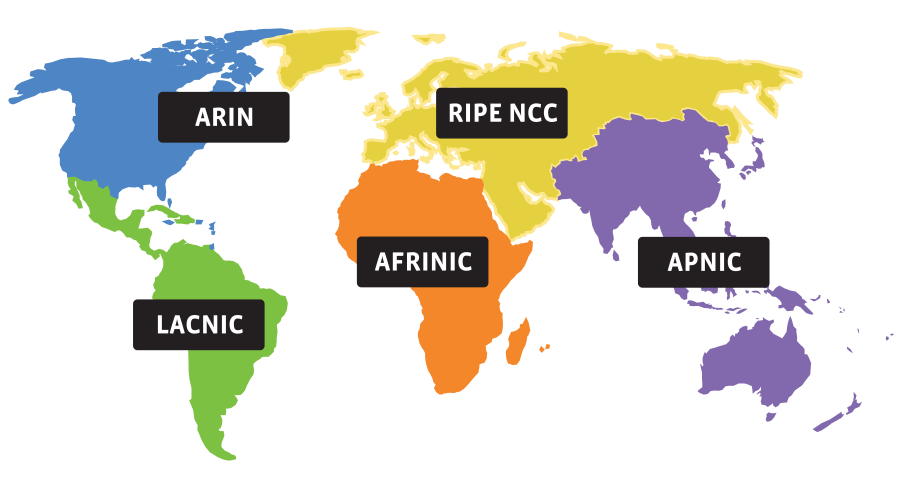
\includegraphics[scale=1.5]{img/rir-map.png} \\
        {\small Fonte: IANA (2020).} 
    \end{figure}
    
%\subsection{Cálculos VLSM}

    Um endereço IPv4 é um número de 32 bits, sendo representado na forma \textit{a.b.c.d/x}, em que \textit{x} é um número inteiro entre 0 e 32 que indica o tamanho do prefixo da rede, o qual representa a quantidade de bits da máscara da rede. Por exemplo, uma máscara 255.255.255.0 é representada por /24. Os $(32 - x)$ bits restantes são os bits dos \textit{hosts}. Essa representação é denominada CIDR (Classless Inter-Domain Routing), uma representação sem classes, adotada após o endereçamento com classes (A, B, C, D e E) cair em desuso devido ao desperdício na alocação de endereços.
    
    Cálculos de VLSM (Variable Length Subnet Masking) operam sobre o CIDR e permitem a criação de sub-redes dentro de uma sub-rede (recursivamente). Por exemplo, um ISP tem uma rede /21 alocada pelo NIC.br e pode dividi-la em sua intranet em 8 sub-redes /24, ou em 4 sub-redes /23 ou até mesmo em 2 sub-redes /23 mais 4 sub-redes /24 de maneira mista.

\subsection{Mitigando a escassez do IPv4 com CGNAT}

    O número de dispositivos conectados à internet tem crescido de tal forma que ultrapassou a capacidade de atendimento de IPs que um ISP pode oferecer aos seus assinantes. Para contrornar isso, a estratégia adotada é, a princípio, oferecer um IP público na interface de saída do roteador de borda (WAN) da sub-rede do cliente e uma faixa de endereços privados na rede local (LAN) do mesmo, sendo feita a tradução de endereços na interface WAN/LAN. IPs privados são blocos definidos pela RFC 1918 e que não devem ser anunciados na internet, sendo restritos ao uso em intranets para o funcionamento do artifício do NAT (network address translation).
    
    Existem ISPs que não possuem endereços o suficiente para todos os assinantes, sendo necessário recorrer ao recurso do CGNAT (Carrier-grade NAT) para contornar o problema. O CGNAT implementa uma camada de NAT na WAN do cliente, deixando de entregar um IP público para alocar um IP privado ao gateway cliente. IPs privados de CGNAT são definidos pela RFC 6598 e é através deles que é implantado o NAT da operadora, em que um mesmo endereço público é compartilhado por vários assinantes.

% \subsection{Motivação para o uso de NAT}
   
   O NAT funciona porque é a camada de transporte a responsável em estabelecer comunicação entre dois hosts e não a camada de rede, isto é, uma porta definida pelos respectivos sistemas operacionais dos hosts garante a conexão fim-a-fim na internet. Assim, a função do IP é rotear os pacotes e do TCP estabelecer a conexão HTTP, por exemplo. Um cliente com IP público dedicado tem a sua disposição 65535 portas, o que lhe daria a possibilidade de estabelecer, teoricamente ao máximo, 65535 conexões simultâneas.
   
   Como no NAT os clientes finais compartilham um único IP público, todas as portas que estão associadas a esse IP serão distribuídas entre eles pelo roteador de NAT, sendo que para cada solicitação de conexão será inserido na tabela de tradução de endereços o par $ ( IP_{publico}, \; Porta_{publica} ) $ associado com o par $ ( IP_{privado}, \; Porta_{privada} ) $ de forma aleatória e não conflituosa caso o par já exista na tabela, dado um tempo de vida para esse vínculo. Essa técnica tradicional de NAT é conhecida como \textit{masquerade}, por mascarar toda rede privada atrás do NAT através de um único IP.
   
\subsection{Aspectos legais quanto ao uso de NAT}
\label{sec:marco_civil}

   Embora a técnica de NAT \textit{masquerade} resolva o problema da escassez de endereços públicos, existe uma particularidade que não pode ser omitida. De acordo com o Art. 13 do Marco Civil da Internet (Lei nº 12.965/2014), ``na provisão de conexão à internet, cabe ao administrador de sistema autônomo respectivo o dever de manter os registros de conexão [...] pelo prazo de 1 (um) ano'', sendo que um registro de conexão é definido pelo ``conjunto de informações referentes à data e hora de início e término de uma conexão à internet, sua duração e o endereço IP utilizado pelo terminal'' \cite{lei12965}. A lei ainda destaca no Art. 22 que um juiz pode ordenar ao ISP o fornecimento dos registros de conexão à internet de um determinado cliente com a finalidade de obtenção de provas para processos judiciais.
   
   Dessa forma, o ISP tem a obrigação legal de manter o rastreio sobre qual IP cada um de seus clientes utilizou para navegar na internet, pois caso ele esteja utilizando a rede para cometer algum crime, a polícia conseguirá encontrá-lo. Isso parte do princípio de que na internet todos devem ser identificados pelo IP como sendo seu endereço virtual, porém o NAT \textit{masquerade} quebra essa identidade por não ser determinístico na tradução do endereço. Por isso, um ISP não pode simplesmente resolver a escassez por IPs utilizando uma metodologia de NAT desenvolvida para redes de escritórios domésticos e de pequenas empresas. No ISP, deve ser utilizada, por questões legais, a técnica específica e determinística chamada de CGNAT, também conhecida como NAT de operadora.

\subsection{Técnicas de CGNAT}

    Existem duas técnicas adotadas na implantação do CGNAT determinístico: o CGNAT horizontal e o vertical. Ambas garantem a operação do NAT, sendo a diferença entre uma e outra simplesmente a metodologia utilizada no mapeamento entre as redes público-privadas e as faixas de porta.
    
    No modelo horizontal, o mapeamento entre os endereços públicos e privados é feito horizontalmente para uma faixa determinada de portas, como é ilustrado na Figura \ref{fig:cgnat_horizontal}, em que o sentido de crescimento numérico dos endereços privados acompanha os endereços públicos. Essa técnica possibilita a implantação simplificada por uso de ferramentas de \textit{netmapping}.
    
    \begin{figure}[!htb]
        \centering
        \caption{Ilustração do modelo de CGNAT horizontal.} 
        \label{fig:cgnat_horizontal} 
        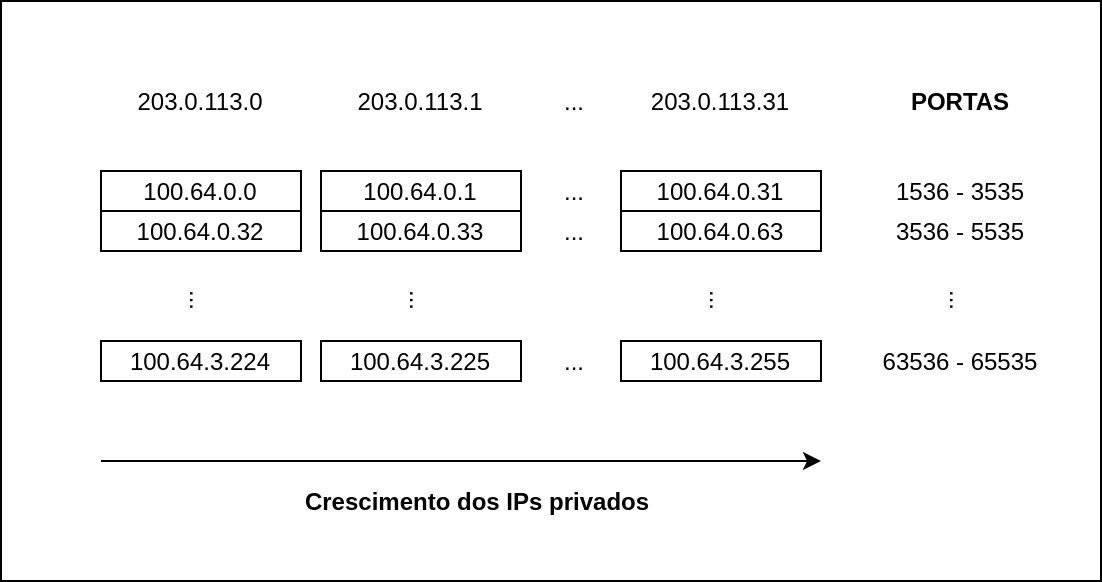
\includegraphics[width=0.9\linewidth]{img/CGNAT-Horizontal.png} \\
        {\small Fonte: do autor (2020).} 
    \end{figure}
    
    No modelo vertical, o sentido de crescimento dos IPs privados não coincide com os IPs públicos, pois o sentido desta vez segue o crescimento do range de portas. Assim, é tomado um IP público como referência e são mapeadas as faixas de portas para os IPs privados consecutivamente, como pode ser visto na Figura \ref{fig:cgnat_vertical}. Essa técnica é de mais fácil entendimento, porém requer mais trabalho para implantação por demandar criação de várias regras individuais de NAT.
    
    \begin{figure}[!htb]
        \centering
        \caption{Ilustração do modelo de CGNAT vertical.} 
        \label{fig:cgnat_vertical} 
        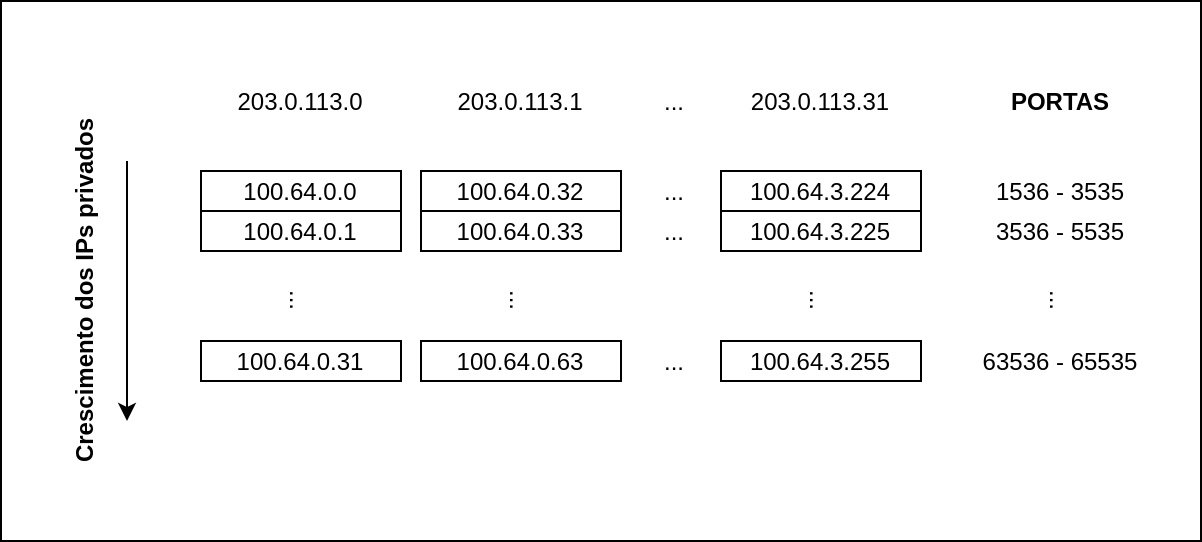
\includegraphics[width=0.9\linewidth]{img/CGNAT-Vertical.png} \\
        {\small Fonte: do autor (2020).} 
    \end{figure}

\subsection{Desvantagens do NAT}

    Apesar de solucionar a escassez de endereços de um ISP, o CGNAT implementa uma camada dupla de NAT para os assinantes, o que não permite o funcionamento de redirecionamentos de portas de maneira simples e direta. O redirecionamento de portas nesse cenário, necessita da compatibilidade do dispositivo adotado para implantação do CGNAT e fica limitado a uma faixa de portas definida pelo mapeamento.
    
    Como consequência do NAT duplo, protocolos P2P não funcionam, pois não existe comunicação de entrada direta com o \textit{host}, sendo necessário o uso de recursos para travessia de NAT, como reversão de conexão ou repasses para aplicação com um nó intermediário para resolução da limitação imposta \cite{kurose2014}.
    
    Do ponto de vista do modelo OSI, o NAT viola o encapsulamento da pilha de protocolos por trabalhar em conjunto nas camadas de rede e de transporte, com a tradução entre IP e porta, sem hierarquia. 
    
\subsection{Migração para IPv6}
    
    Como solução aos problemas estruturais e operacionais do NAT, foi proposta a migração para o IPv6 (IP versão 6), que adota como endereço um número de 128 bits, muito mais do que o suficiente para endereçar unicamente todos os dispositivos em LAN sem o uso de IPs privados. Como todos os dispositivos podem ter um IP público através do IPv6, não é necessário o conceito de NAT com o novo protocolo.
    
    Embora o IPv6 seja a solução, não basta apenas o ISP implantá-lo, é necessário que o acordo de tráfego no novo protocolo também esteja fechado com os servidores de sistemas e de provedores de conteúdo. Enquanto isso não for um tecnologia de ponta-a-ponta, o CGNAT é um modelo satisfatório no processo de transição.

\section{Segurança de ambientes de rede}

    Sistemas em rede estão suscetíveis a ataques, pois a internet é promíscua por sua própria natureza. O objetivo da segurança é minimizar os riscos, pois não existe sistema 100\% seguro. A cada dia são descobertas novas falhas e as correções também evoluem de forma constante.
    
    A segurança da informação é regida por quatro pilares: autenticidade, confidencialidade, integridade e disponibilidade. A segurança de redes tem seu foco principal em disponibilidade, prezando pela minimização de vulnerabilidades que possam ser exploradas para causar interrupção no serviço, sejam exploradas através de falhas físicas ou através de ataques de negação de serviço.
    
    Entre as principais ferramentas de defesa disponíveis para segurança de rede, estão o firewall e a VPN (Virtual Private Network), que serão descritas a seguir.

\subsection{Firewall}

    Firewall é um ponto entre duas ou mais redes onde é possível controlar todo o tráfego de dados que passa através dele. Assim, esse ponto único constitui um mecanismo utilizado para proteger uma rede confiável de uma rede pública não-confiável \cite{nakamura2007}.
    
    As técnicas básicas de firewall são a filtragem de pacotes estática (\textit{stateless}) e a filtragem de pacotes baseada em estados (\textit{stateful}). No firewall \textit{stateless}, as regras são aplicadas na camada de rede (camada 3) e de transporte (camada 4), sendo feita a filtragem a partir das informações de IP, porta e protocolo contidas no cabeçalho do pacote. A técnica \textit{stateless} apresenta alto desempenho e performance para gerenciamento de tráfego devido a sua simplicidade. Em contrapartida, não é uma técnica suficiente para filtragem de serviços de portas dinâmicas, em que as portas de comunicação são definidas em tempo de execução, como nos protocolos RPC e FTP \cite{nakamura2007}. O problema das portas dinâmicas é possível de ser tratado com um firewall \textit{stateful}, que mantém registros das conexões para filtragens mais inteligentes e dinâmicas, tendo como custo um maior consumo de recursos de processamento.
    
    As vulnerabilidade de obtenção de informação, em que atacantes oportunistas podem conseguir informações em banners de protocolos de rede local expostos na internet, podendo conseguir informações valiosas para auxiliar em um ataque de invasão, podem ser tratadas com firewall pelo uso de regras de acesso definidas por IP. Além disso, a vulnerabilidade de invasão também pode ser corrigida com um firewall fazendo bloqueio de portas aos invasores. 

    O bloqueio de portas também auxilia na minimização de ataques de negação de serviço, pois um atacante pode conseguir amplificar o tráfego e congestionar a rede explorando protocolos como DNS e SSDP, que têm o pacote de resposta muito maior que a requisição, podendo inundar a rede em um ataque coordenado. Com as portas desses serviços fechadas àqueles que não necessitam acessá-las, mais segurança é agregada à rede.
    
    O firewall não é a solução total para segurança da rede. É fundamental selecionar os usuários que podem acessar a rede e definir os seus respectivos níveis de acesso (somente leitura ou leitura e escrita). A autenticação e a autorização são também importantes aspectos a serem implementados na infraestrutura de segurança \cite{nakamura2007}.

\subsection{VPN}

    Uma VPN tem como funcionalidade prover conexão a uma rede local através da internet por meio de um túnel de conexão criptografado. O mecanismo da VPN provê serviço de acesso remoto como também serve de mecanismo para controle de acesso, fornecendo uma camada de autenticação à rede interna e de autorização quando combinada com um firewall.
    
    Os conceitos que fundamentam a VPN são a criptografia e o tunelamento. A criptografia é utilizada para garantir a autenticidade, o sigilo e a integridade dos dados através da conexão, e é a base da segurança dos túneis VPN \cite{nakamura2007}. Uma VPN implantada com protocolo PPTP ou L2TP garante somente autenticidade, enquanto IPSec e protocolos baseados em TLS (como Stunnel e aplicações modernas de VPN) somam integridade e confidencialidade ao túnel.

\section{Topologia de um ISP}

    O modelo comum de topologia adotado por operadoras de internet é formado por um triângulo entre roteadores B-RAS (\textit{broadband remote access server}), CGNAT e borda, conforme Figura \ref{fig:isp}. Os clientes finais conectam-se à rede através de PPPoE ao roteador B-RAS, que por sua vez encaminha o tráfego de IP público à borda que será roteada para a internet. Tráfego de IP privado de CGNAT (RFC 6598) é encaminhado ao equipamento que traduz os IPs privados em públicos antes de serem roteados à internet pela borda.
    
    Dependendo da dimensão da rede, é possível adotar modelos simplificados para economia de recursos, fazendo a mescla das funções de um ou de mais equipamentos em um único, desde que o equipamento suporte essa configuração.
    
    A Figura \ref{fig:isp} é uma representação genérica de camada 3 do núcleo da rede de um ISP. Existem muitos outros elementos de conexão de camada 2 e de camada 1 (lógica e física respectivamente) entre os dispositivos que não estão na imagem, como enlaces de rádio ou de fibra óptica. Também foi omitido, por simplificação, que dentro do salto entre o ABR e a Internet na Figura \ref{fig:isp}, existe o ASBR (Autonomous System Border Router), que é resposável por rotear o tráfego para a internet.
    
    \begin{figure}[!htb]
        \centering
        \caption{Modelo de topologia de um ISP.} 
        \label{fig:isp} 
        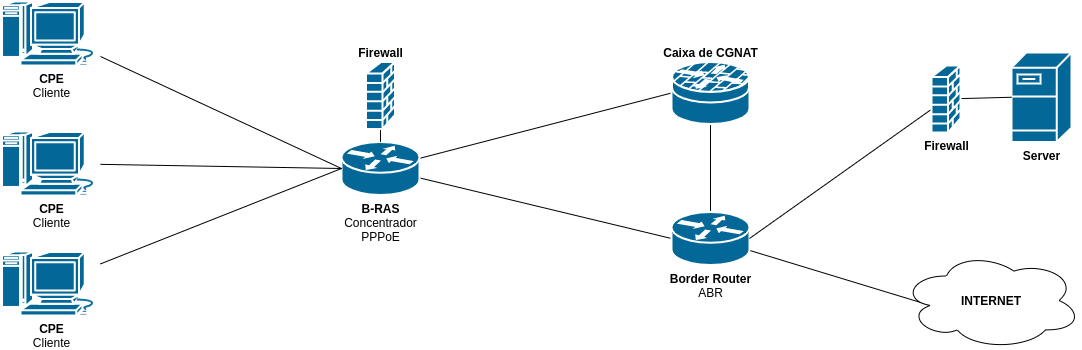
\includegraphics[width=0.9\linewidth]{img/isp.png} \\
        {\small Fonte: do autor (2020).} 
    \end{figure}
    
    Na infraestrutura lógica do ISP, também entram os servidores de serviços locais, que provêm servidores de autenticação RADIUS, serviço de DNS local para respostas mais rápidas, Proxy HTTP\footnote{Também conhecido como CDN -- content distribution network.} para poupar consumo de banda de acesso à internet e serviço de VPN.
    
  \chapter{ENDEREÇAMENTO IP}
\label{cap:enderecamento}

    O endereço IP é a identificação que possibilita o tráfego de dados desde sua origem até o destino através da rede mundial de computadores, por isso é necessário fornecer endereços IP para todos os dispositivos que se conectam à internet. Em um provedor, a rede (que utiliza um conjunto de IPs com mesmo prefixo) é dimensionada de acordo com a quantidade de clientes que serão atendidos dentro de uma determinada área de abrangência, que geralmente é atomizada por cidades.

\section{Rede IP da Minasnet}
    
    Na Minasnet, a rede é subdividida em áreas OSPF, sendo que cada área é associada a uma cidade. Zonas rurais e vilarejos recebem o mesmo código de área da cidade a qual pertencem. Assim, a sub-rede é dimensionada de acordo com o tamanho da cidade e com a quantidade de clientes associados àquela área. Geralmente, um bloco /24 de endereços é o menor espaço de endereçamento atribuído a uma área e um bloco /22 é o maior. Por exemplo, a franquia de Perdões tem uma rede /22, isso significa que existem 1024 endereços públicos dedicados para atendimento aos clientes dessa cidade.
    
   Os IPs são associados aos CPEs (dispositivo \textit{gateway} da rede interna de um cliente) através de um túnel PPPoE fechado com o concentrador (B-RAS). Como o próprio nome sugere, o concentrador centraliza todas as conexões de camada 3 dos clientes conectados em um único equipamento. Entretanto, dependendo do hardware e da configuração do software de um equipamento concentrador, pode ser necessário a utilização de mais de um equipamento para dividir a carga do servidor PPPoE. 
   
   Na Minasnet, um exemplo disso foi a franquia de Oliveira, uma das mais recentemente atendidas pelo ISP. A princípio existia um único concentrador PPPoE que, devido à demanda de clientes entrantes, teve sua carga dividida com um segundo concentrador instalado junto a ele. O padrão atual da empresa é manter no máximo 1024 clientes em um único concentrador.
   
   Para documentar a rede IP do AS (conjunto de todas as sub-redes públicas de um ISP), é utilizado o software PHPIPAM\footnote{PHPIPAM \url{https://phpipam.net} é um software \textit{open-source} de gerenciamento de endereços de rede (IP, VLAN e etc.).}. Neste software é possível criar o aninhamento entre sub-redes e deixar descrito qual a finalidade de cada uma delas, facilitando consultas e manipulações de VLSM nessas redes dentro do próprio sistema. Tomando o exemplo de Perdões, no PHPIPAM existe uma rede com mesmo nome da cidade, na qual estão documentados todos os IPs públicos da rede /22 dimensionada para a mesma, além dos IPs privados utilizados na franquia, que estão contidos nas redes 10.0.0.0/8, 172.16.0.0/12 e 192.168.0.0/16, definidas pela RFC 1918 \cite{rfc1918}, e o espaço compartilhado 100.64.0.0/10 definido pela RFC 6598 \cite{rfc6598}. Dentro da rede IP pública, é reservada uma sub-rede para alocação de IP fixo e o restante dos IPs são alocados dinamicamente para os clientes.
   
   Dado que a franquia de Perdões possui muito mais do que 1024 clientes, um \textit{pool}\footnote{Diferente de uma rede, que tem reservado o primeiro e o último endereço para o \textit{host} e para o \textit{broadcast} respectivamente, no \textit{pool} todos os endereços são alocados, inclusive 0 e 255.} de prefixo /22 não atenderia à demanda. A solução para a escassez de endereços na franquia é a utilização do artifício do NAT, disponibilizando IPs privados aos clientes e fazendo associação do par IP-porta com o IP público de destino do NAT. Redes privadas não devem ser anunciadas na internet pública e a única forma de comunicarem-se com o mundo é através do NAT. 
   
\section{Metodologia para implementação de CGNAT}

   Observando os requisitos definidos pelo Art. 13 da Lei nº 12.965/2014, descritos na Seção \ref{sec:marco_civil}, e relacionando-os com a infraestrutura de um concentrador, devemos registrar o \textit{timestamp} de início e de fim da sessão PPPoE do cliente bem como qual o IP foi disponibilizado a ele durante essa sessão. A sessão PPPoE inicia-se no instante em que o cliente estabelece conexão e se encerra quando acontece a desconexão. Salvar essas informações é simples quando se utiliza um servidor RADIUS\footnote{A Minasnet utiliza o FreeRADIUS \url{https://freeradius.org}.}, pois a função básica desse serviço é autorizar a conexão de assinantes, atribuindo IP e armazenando o \textit{log} das informações de acesso. 

   A RFC 6888 estabelece requisitos para implementação do CGNAT de maneira segura. Um ponto importante dessa RFC é a definição obrigatória do mapeamento direto entre os \textit{pools} de endereços públicos e privado, imprescindível para que o CGNAT seja determinístico. Outro ponto importante é a manutenção de registro das informações do assinante conectado, assim como especificado pelo Marco Civil da Internet.
   
   Embora a RFC 6888 esteja em consonância com o Marco Civil da Internet, existe divergência. A diferença é que o Marco Civil estabelece normas tipicamente orientadas para provedores que entregam somente IP público para seus clientes, por não estabelecer uma regra de registro de número de porta nas conexões. A RFC 6888 é mais ampla por contemplar as necessidades de registro de conexões através de CGNAT para garantir o rastreio da identidade dos clientes na internet, definindo como parâmetros para \textit{log} \cite{rfc6888}:
   
   \begin{enumerate}[label=\alph*)]
       \item o protocolo de transporte;
       \item o IP interno;
       \item o IP externo de origem;
       \item a porta externa de origem;
       \item o \textit{timestamp} de registro.
   \end{enumerate}

   Vale ressaltar que IP externo de origem e porta externa de origem são valores do lado do provedor, sendo que IP de destino e porta de destino seriam do lado da aplicação. Não é recomendado armazenar informações de destino dos pacotes, uma vez que isso quebraria a privacidade de navegação dos assinantes por rastrear tudo que eles tem acessado na internet \cite{rfc6888}.

   O problema de se seguir à risca os cinco parâmetros definidos acima é que demandaria muito espaço em disco para a manutenção do rastreio das conexões, pois seria necessário armazenar no banco de dados de \textit{log} cada novo registro na tabela de tradução de endereços. Seria um volume tão grande de dados que até uma consulta para atender a uma solicitação judicial poderia ser demorada, lembrando que o banco de dados deve manter por 1 ano todas as informações.

   A solução desse problema é utilizar técnicas que fazem mapeamento direto entre uma faixa contígua de portas, de tamanho padronizado, para os IPs públicos e privados. Com o mapeamento de portas, só é necessário registrar em \textit{log} o IP interno do cliente e os \textit{timestamps} de início e de fim da sessão PPPoE, resultando em uma redução considerável no volume de dados, pois serão somente três campos registrados ao invés dos cinco. 
 
   Outra melhoria para redução do volume de dados é utilizar dois campos de \textit{timestamp} ao invés de um só -- um para o momento de conexão e outro para o de desconexão. Assim, a inserção de novas linhas na base de dados será necessária somente quado o cliente conectar, inserindo o \textit{timestamp} no campo de conexão e deixando o de desconexão \textit{null} enquanto o cliente estiver conectado. No momento da desconexão, basta atualizar o campo \textit{null} com a data e hora da desconexão.
 
   Apesar de o mapeamento de portas não gerar alto volume de dados de \textit{log} de conexão dos assinantes, para que seja uma técnica suficiente na implementação do CGNAT é preciso manter documentadas as regras de mapeamento de IP-porta. A utilização de uma planilha é a maneira mais prática para realizar tal tarefa. Na Minasnet, é mantida uma planilha na qual as informações são registradas de acordo com colunas contendo:

   \begin{enumerate}[label=\alph*)]
       \item nome do concentrador alvo do CGNAT;
       \item nome da franquia;
       \item sub-rede interna;
       \item sub-rede externa;
       \item \textit{timestamp} de início de vigência da regra.
       \item anotações.
   \end{enumerate}
   
   Os dois primeiros itens são apenas por questão de organização, pois existem dezenas de concentradores no ISP e todos estão documentados nessa planilha, sendo somente as informações de mapeamento de redes interna e externa e o \textit{timestamp} relevantes para eficácia do registro. As anotações tem informações sobre desativação da regra de CGNAT ou modificações nas redes, não sendo criado mais campos específicos porque o objetivo é que seja alterado o mínimo possível. Até hoje, poucas vezes houve alterações no mapeamento das sub-redes. O Quadro \ref{tab:planilha_cgnat} exemplifica o uso da planilha para controle e documentação dos mapeamentos.

   \begin{quadro}[htb]
        \begin{center}
            \caption{Exemplo de planilha para controle de CGNAT.} 
            \label{tab:planilha_cgnat}
            \vspace{0.2cm}
        \footnotesize
            \begin{tabular}{|c|c|c|c|c|c|}
            \hline
            Concentrador & Franquia & Rede interna & Rede externa & Início & Anotações \\
            \hline
            \hline
            CON-PER-01 & Perdões & 100.64.0.0/22 & 203.0.113.0/27 & 2019-04-18 17:15 & Vigente \\
            CON-PER-02 & Perdões & 100.64.4.0/22 & 203.0.113.32/27 & 2019-05-02 12:05 & Vigente \\
            CON-PER-03 & Perdões & 100.64.8.0/22 & 203.0.113.64/27 & 2019-11-13 16:35 & Vigente \\
            \hline 
            \end{tabular}
        \end{center}
        \centering{\small Fonte: do autor (2020).} 
    \end{quadro}


    A Minasnet adota por padrão a disponibilização de 2.000 portas para cada cliente atrás do CGNAT, definindo o intervalo da faixa entre 1536 e 65535. Isso significa que, para cada IP público do CGNAT do ISP, existem 32 clientes internos conectados à internet através dele. Esse dimensionamento de 1 IP externo para 32 internos denomina a razão de compartilhamento 1:32. As portas de uso reservado (0-1023) não são usadas e a numeração começa a partir de 1536 por questões de arredondamento de cálculos.
    
    Os cálculos a seguir demonstram o dimensionamento do mapeamento de portas descrito. O primeiro passo é verificar a quantidade de portas $ \Delta $ que estão sendo dedicadas ao CGNAT por um único IP, simplesmente subtraindo os limites de portas definidos e somando 1, pois a primeira porta também é contabilizada:

    \begin{equation}
        \Delta = porta_{maior} - porta_{menor} + 1
               = 65535 - 1536 + 1
               = 64000
    \end{equation}
    
    O que resulta em 64.000 portas. Como cada IP interno tem 2.000 portas mapeadas para ele, então a quantidade de IPs internos $ n $ para cada IP público será:

    \begin{equation}
        n = \frac{64000}{2000}
          = 32
    \end{equation}

    Como dito anteriormente, um concentrador da Minasnet normalmente é dimensionado para atender até 1024 clientes. De acordo com a proporção 1:32, são necessários 1024 IPs internos e 32 IPs externos  para implementação do CGNAT nesse caso. A quantidade de IPs externos é obtida tirando a razão 1024 por 32, pois a razão de compartilhamento dada é 1:32, o que resulta em 32 IPs. Então, nesse concentrador deve ser criado uma mapeamento de uma rede interna com 1024 endereços (/22) para uma rede externa de 32 endereços (/27).
    
    Calcular mapeamentos para outros prefixos de rede é simples, pois seguem a mesma lógica usada no mapeamento /22 entre /27. O Quadro \ref{tab:netmap} mostra alguns dos mapeamentos que são possíveis de serem feitos seguindo a metodologia usada aqui. A demonstração pode ser feita alterando os valores correspondentes dos cálculos supracitados, em sempre será obtida a razão constante de 1:32 entre IP externo e interno.

    \begin{quadro}[htb]
        \begin{center}
            \caption{Mapeamento direto entre sub-redes internas/externas usando CGNAT 1:32.} 
            \label{tab:netmap}
            \vspace{0.2cm}
            \footnotesize
            \begin{tabular}{|c|c|c|}
            \hline
            Prefixo privado & Prefixo público & Quantidade de clientes \\
            \hline
            \hline
            ... & ... & ... \\
            /20 & /25 & 4096 \\
            /21 & /26 & 2048 \\
            /22 & /27 & 1024 \\
            /23 & /28 & 512 \\
            /24 & /29 & 256 \\
            /25 & /30 & 128 \\
            /26 & /31 & 64 \\
            /27 & /32 & 32 \\
            \hline 
            \end{tabular}
        \end{center}
        \centering{\small Fonte: do autor (2020)} 
    \end{quadro}

\subsection{Implementação de CGNAT no RouterOS}

    Até aqui, foi fundamentada a metodologia utilizada para o CGNAT. Nesta seção, será apresentada a implementação das regras em roteadores MikroTik através do sistema operacional embarcado RouterOS\footnote{RouterOS \url{https://mikrotik.com/software} é o sistema operacional nativo dos equipamentos MikroTik, sendo um software proprietário com \textit{kernel} Linux.}, com geração das regras através de ferramenta desenvolvida em Python de autoria própria.
    
    %\footnote{Python \url{https://www.python.org/} é uma linguagem de programação interpretada e multiplataforma.}.
    
    O primeiro passo para o desenvolvimento prático do CGNAT é entender o que o RouterOS nos proporciona para atingir esse objetivo. Por ser baseado em Linux, a ideia básica é construir as regras de NAT através do módulo de firewall do sistema, pois o NAT é interpretado como uma regra de firewall por fazer modificação no cabeçalho dos pacotes de dados ao alterar os valores de endereço e de porta originais.

    O módulo utilizado é a tabela NAT do firewall do RouterOS, sendo necessário configurar os seguintes parâmetros na geração das regras conforme definidos na documentação \cite{natmikrotik}:

    \begin{enumerate}[label=\alph*)]
        \item \label{nat:action} {\tt action}, especifica a ação que deve ser executada; neste caso, a ação definida foi o {\tt netmap}, que consiste no mapeamento direto entre as redes interna e externa;
        
        \item \label{nat:chain} {\tt chain}, é configurado como {\tt srcnat}, pois os pacotes alvos da regra originam-se na rede interna ao firewall; 
        
        \item \label{nat:protocol} {\tt protocol}, são configurados tanto TCP e UDP individualmente; 
        
        \item \label{nat:srcaddress} {\tt src-address}, é a sub-rede interna;
        
        \item \label{nat:toaddress} {\tt to-addresses}, é a sub-rede externa;
        
        \item \label{nat:toports} {\tt to-ports}, é a faixa de portas do IP público alocada.
    \end{enumerate}

    A única ressalva é que, para o pleno funcionamento do NAT para pacotes de protocolos de camada 3 (ICMP), devem ser criadas regras em que não estejam definidos os itens (\ref{nat:protocol} e (\ref{nat:toports}.

    Com os parâmetros definidos, o template do comando a ser executado na CLI é dado conforme o exemplo da Figura \ref{fig:netmap_cli}. O método de utilização simplificada do {\tt netmap} foi obtido de \cite{maia2018} e é uma técnica de CGNAT horizontal, ilustrada na Figura \ref{fig:cgnat_horizontal}. Neste exemplo, são utilizadas as sub-redes indicadas no exemplo do CON-PER-01 no Quadro \ref{tab:planilha_cgnat}. Pode-se notar que foi utilizado um prefixo /27 ao invés de um /22 no comando, isso acontece porque para que a regra de {\tt netmap} faça o mapeamento direto, as redes devem ter o mesmo prefixo para que a correspondência entre os IPs seja possível. Assim, uma rede /22 deve ser subdividida em 32 sub-redes /27 para que seja feito o mapeamento com uma rede pública de prefixo /27. Para fazer o casamento entre outros valores de prefixos, o princípio é o mesmo.

    \begin{figure}[!htb]
        \centering
        \caption{Template do comando de configuração de netmap no RouterOS.} 
        \label{fig:netmap_cli}
        
        \begin{Verbatim}[fontsize=\small]
            /ip firewall nat 
                add action=netmap           \
                chain=srcnat                \
                protocol=tcp                \
                src-address=100.64.0.0/27   \
                to-addresses=203.0.113.0/27 \
                to-ports=1536-3535          \
                disabled=yes
        \end{Verbatim} 

        {\small Fonte: do autor (2020).} 
    \end{figure}

    
    
    Acontece que, fazer geração manual de todas essas regras é um trabalho extenso e cansativo, que pode ficar sujeito a falhas humanas. Para isso, foi desenvolvido um utilitário de CLI para geração das regras para construir {\tt netmap} entre qualquer prefixo, desde que respeite a razão 1:32. O software foi desenvolvido em Pyhton.%, o que permite que seja usado em qualquer sistema operacional que tenha o ambiente de execução Python instalado.

    O fundamento utilizado na construção do programa baseia-se na geração de uma árvore binária oriunda das subdivisões recursivas de uma rede privada de determinado prefixo, situada na raiz, até que chegue em uma camada em que as folhas tenham o mesmo prefixo que a rede pública, procedimento ilustrado na Figura \ref{fig:arvore_binaria}. A partir daí, o algoritmo obtém uma lista com todas as sub-redes formadas pelas folhas dessa árvore, e gera as regras de {\tt netmap} conforme definido no template da Figura \ref{fig:netmap_cli}, incrementando o número de portas em um valor fixo de 2.000. 
    
    \begin{figure}[!htb]
        \centering
        \caption{Árvore binária das subdivisões recursivas de um /22 até um /25.}
        \label{fig:arvore_binaria}
        
        \small
        \begin{tikzpicture}[->,>=stealth',level/.style={sibling distance = 7cm/#1,
  level distance = 1.5cm}] 
            \node {/22}
            child {
                node {/23}
                child {
                    node {/24}
                    child {
                        node {/25}
                        node {/25}
                    }
                    child {
                        node {/25}
                        node {/25}
                    }
                }
                child {
                    node {/24}
                    child {
                        node {/25}
                        node {/25}
                    }
                    child {
                        node {/25}
                        node {/25}
                    }
                }
            }
            child {
                node {/23}
                child {
                    node {/24}
                    child {
                        node {/25}
                        node {/25}
                    }
                    child {
                        node {/25}
                        node {/25}
                    }
                }
                child {
                    node {/24}
                    child {
                        node {/25}
                        node {/25}
                    }
                    child {
                        node {/25}
                        node {/25}
                    }
                }
            };
        \end{tikzpicture}

        {\small Fonte: do autor (2020).} 
    \end{figure}
    
    A ferramenta desenvolvida foi nomeada como {\tt py-cgnat}. O código-fonte está disponível no GitHub\footnote{\url{https://github.com/williamabreu/py-cgnat}.} do autor e o executável pode ser baixado através do repositório oficial do Python\footnote{\url{https://pypi.org/project/pycgnat/}.}. O software foi desenvolvido seguindo as convenções do ecossistema Python e é \textit{open--source}, sendo lançado sob licença permissiva MIT para garantir liberdade de uso e de distribuição sem complicações. A versão 1.0b1 é a utilizada neste trabalho.
    
    
\subsection{Utilização do utilitário py-cgnat}
    
    A seguir, será utilizado o mapeamento do concentrador CON-PER-01 (conforme Quadro \ref{tab:planilha_cgnat}) para exemplificar o uso do programa {\tt py-cgnat} via terminal de comando. Para fazer a geração das regras de {\tt netmap} para RouterOS, o comando a ser executado no terminal segue conforme mostrado na Figura \ref{fig:pycgnat_gen}. Devem ser informados os seguintes parâmetros: a rede privada e a pública, a opção {\tt gen} para acionar o módulo de geração e a plataforma onde será configurado o CGNAT, que neste caso é o RouterOS. O último parâmetro é opcional e é o nome do arquivo de destino das regras caso queira ser salvo, pois se deixado em branco, as regras serão impressas no próprio terminal de comando. O campo plataforma foi posto por questão de extensibilidade, para deixar o software pronto para futuras novas versões, em que se pretende suportar equipamentos de outros fabricantes.
    
    \begin{figure}[!htb]
        \centering
        \caption{Exemplo de uso do programa py-cgnat para geração de CGNAT para RouterOS.} 
        \label{fig:pycgnat_gen}
        
        \begin{Verbatim}[fontsize=\small]
            In: pycgnat 100.64.0.0/22 203.0.113.0/27 gen routeros rules.rsc
            Out: null
        \end{Verbatim} 

        {\small Fonte: do autor (2020).} 
    \end{figure}
    
    O programa também calcula as traduções entre IP público-privado através do módulo {\tt trans}. Um exemplo é uma consulta para o IP privado 100.64.0.47, que retorna o IP público 203.0.113.15 e a faixa de portas definida entre 3536 e 5535 com o comando da Figura \ref{fig:pycgnat_transd}. De maneira reversa, uma consulta para o endereço 203.0.113.15 na porta 5000 retorna o cliente com IP 100.64.0.47, que pode ser verificada conforme Figura \ref{fig:pycgnat_transr}. As consultas de traduções independem de plataforma, pois fazem parte da lógica da metologia de mapeamento de portas utilizada. 
    
        \begin{figure}[!htb]
        \centering
        \caption{Exemplo de uso do programa py-cgnat para traduções de IP privado para público.} 
        \label{fig:pycgnat_transd}
        
        \begin{Verbatim}[fontsize=\small]
            In: pycgnat 100.64.0.0/22 203.0.113.0/27 trans -d 100.64.0.47
            Out: {"public_ip": "203.0.113.15", "port_range": [3536, 5535]}
        \end{Verbatim} 

        {\small Fonte: do autor (2020).} 
    \end{figure}
    
     \begin{figure}[!htb]
        \centering
        \caption{Exemplo de uso do programa py-cgnat para tradução de IP público para privado.} 
        \label{fig:pycgnat_transr}
        
        \begin{Verbatim}[fontsize=\small]
            In: pycgnat 100.64.0.0/22 203.0.113.0/27 trans -r 203.0.113.15:5000
            Out: {"private_ip": "100.64.0.47", "port_range": [3536, 5535]}
        \end{Verbatim} 

        {\small Fonte: do autor (2020).} 
    \end{figure}
    
    Além disso, o software foi desenvolvido para também ser utilizado como biblioteca de programação, com o objetivo de automatizar processos utilizando Python ou de integrar com sistemas já existentes, caso haja necessidade. Uma breve documentação (em inglês) do uso pode ser obtida no Apêndice A ou nos repositórios do {\tt py-cgnat} no GitHub ou no PyPI.
 
\section{Considerações sobre o uso de CGNAT}
    
    Uma ressalva para o processo de consulta das traduções de endereços é que, caso seja necessário descobrir qual cliente estava navegando com determinado IP em um determinado instante, é necessário consultar no banco do RADIUS qual o \textit{login} PPPoE esteve com aquele IP no dado momento. Esse tipo de solicitação acontece geralmente por ordem judicial ao ISP, a fim de descobrir a identidade de criminosos, que atuam na internet ou através dela.
    
    É muito importante seguir a documentação exemplificada na planilha do Quadro \ref{tab:planilha_cgnat} para garantir o cumprimento do Marco Civil da Internet. Por isso, a utilização de faixas de endereços distintas para clientes com dívida, denominado \textit{pool} de bloqueio, é considerada uma má prática quando não aplicada a técnica de CGNAT em clientes com velocidade de navegação reduzida, porque no período de bloqueio por dívida, seria impossível fazer rastreamento por IP. 

\subsection{Dificuldades encontradas na implantação}
    
    A dificuldade encontrada no \textit{deploy} do CGNAT foi que dois concentradores não estavam com a tabela NAT do firewall funcionando, sendo que o motivo da falha era desconhecido pela equipe. A solução foi subir as regras no dispositivo do ABR, pois como eram poucos clientes, as regras da rede do CGNAT não impactou o desempenho do roteador de borda, sendo feito acompanhamento de consumo de CPU durante momentos de pico do dia (por volta de 20h) para constatar isso. Outra fonte de constatação foi a ausência de reclamações por clientes daquela área onde foi aplicada essa solução de contorno. Também é possível colocar roteadores MikroTik dedicados ao CGNAT intermediando concentrador e borda, mas não foi adotada esta técnica como finalidade do trabalho.
    
  \chapter{SEGURANÇA DE REDE}

    Estar conectado à internet requer cuidados, pois dispositivos expostos à rede pública estão sujeitos às ameças de segurança que podem atacá-los. Sistema completamente seguro não existe, mas usuários finais devem tomar os devidos cuidados em suas redes locais bem como os ISPs também devem tomar as medidas que estiverem ao alcance. No ISP, as competências de segurança atribuídas ao NOC são manter seguros os serviços, protocolos e as redes de telecomunicações, que estão nos níveis mais baixos da implementação das políticas de segurança da informação, enquanto o desenvolvimento de software e interação humano-computador estão em alto nível. A segurança é um acordo que deve ser cumprido por todas as partes em todos os níveis para minimização dos incidentes.

\section{IP Blacklist}

    A Minasnet, como sendo um AS, tem delegação sobre vários blocos de IP que dão aos seus assinantes identidade na internet. O primeiro problema quanto à segurança surge neste ponto, pois a conectividade traz riscos, que se iniciam pelo IP público por onde os ataques conseguem propagar-se pela internet (ou pela intranet, via rede privada).
    
    Grande parte dos \textit{worms} são propagados pela internet através de \textit{spam}, que são enviados de maneira massiva por dispositvos infectados, sejam computadores, smartphones, roteadores domésticos e até roteadores de \textit{core}, basta ter conexão à internet que se torna vulnerável a \textit{botnets}. Assim, uma forma de controlar o envio de spam, por parte dos provedores de serviço, é a utilização de listas negras com IPs que foram identificados como fonte de envio de \textit{spam}.
    
    Chamadas de \textit{Real-time Blackhole List} (RBL), doravante \textit{blacklist}, proporcionam a listagem de IPs detectados recentemente como participantes ativos de \textit{botnet} para envio de \textit{spam}, possibilitando ao provedor de serviço bloquear todo o tráfego de e-mail a partir daquele endereço IP listado. 
    
    Neste trabalho, o uso de RBL tem sua finalidade para monitoramento de IPs do AS que estão listados na blacklist, com o objetivo de identificar infecções no núcleo da rede (devido à vulnerabilidades associadas à equipamentos MikroTik com IP público), bem como nos assinantes. Para isso, foi utilizado o Composite Blocking List (CBL)\footnote{CBL \url{https://www.abuseat.org} é uma divisão da Spamhaus.}, uma RBL com consula no padrão DNS Blacklist (DNSBL).
    
    DNSBL é informado pela RFC5782, funcionando com estrutura semelhante a um DNS reverso. Cada IP listado em uma DNSBL tem um subdomínio correspondente, sendo que cada entrada de subdomínio é criada revertendo os octetos do IP e concatenando com o domínio da DNSBL. Uma consulta à DNSBL retorna no registro {\tt A} o endereço 127.0.0.2 e no registro {\tt TXT} a descrição do motivo pelo qual o IP está listado na \textit{blacklist} \cite{rfc5782}. Quando o IP não está na \textit{blacklist}, a consulta retorna o erro {\tt NXDOMAIN}. Por exemplo, uma consulta para verificar se o IP 192.0.2.99 está listado na CBL seria feita a partir da entrada 99.2.0.192.cbl.abuseat.org e, em caso de listagem positiva, o link informado no registro {\tt TXT} daria um relatório detalhado da origem e qual tipo de infecção foi detectada atrás desse IP. Em terminal de comando Linux, a consulta pode ser feita da seguinte forma, para os registros {\tt A} e {\tt TXT}, respectivamente, conforme Figura \ref{fig:dnsbl_query}.
    
    \begin{figure}[!htb]
        \centering
        \caption{Exemplo de consulta à DNSBL CBL via terminal Linux.} 
        \label{fig:dnsbl_query}
        
        \begin{Verbatim}[fontsize=\normalsize]
            host -t A 99.2.0.192.cbl.abuseat.org
            host -t TXT 99.2.0.192.cbl.abuseat.org
        \end{Verbatim} 

        {\small Fonte: do autor (2020).} 
    \end{figure}
    
    O monitoramento foi feito de maneira automatizada, através de um simples programa feito em Python para fazer a varredura de todos os blocos de IP do AS, que até o momento é constituído por 8.192 endereços. O programa varre todos os endereços e retorna um resumo contendo somente aqueles que estão listados na \textit{blacklist}, que serão analisados através do relatório detalhado na página da CBL.
    
    O Gráfico \ref{fig:plot_blacklist} mostra o resultado do monitoramento de IPs da Minasnet listados na CBL entre abril e setembro de 2019 e o Anexo A é um exemplo de relatório detalhado fornecido pela plataforma, contendo informações de origem, destino e tipo de infecção detectada pelo \textit{honeypot}, além de sugestões para correção do problema.
    
    \begin{grafico}[!htb]
        \centering
        \caption{Contagem de IPs do AS listados na CBL entre abril e setembro de 2019.} 
        \label{fig:plot_blacklist} 
        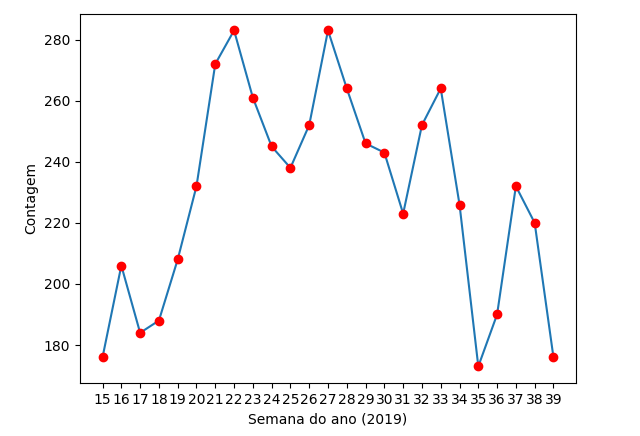
\includegraphics[scale=0.5]{img/plot_blacklist.png} \\
        {\small Fonte: do autor (2020).} 
    \end{grafico}
    
    \textit{Honeypots} são máquinas que emulam determinados sistemas operacionais e serviços, para que um atacante interaja com ela sem que perceba que está entrando em uma armadilha \cite{spampots2007}. É utilizando deste artifício que a CBL faz a detecção de \textit{botnets} e registra o IP de origem do \textit{spam}, sendo a Figura \ref{fig:honeypot} um exemplo de arquitetura utilizada para essa detecção. A descrição da metodologia utilizada pela plataforma pode ser obtida (em inglês) no site da CBL, já referenciado em nota de rodapé. 
    
    \begin{figure}[!htb]
        \centering
        \caption{Arquitetura de um honeypot para detecção de spam.} 
        \label{fig:honeypot} 
        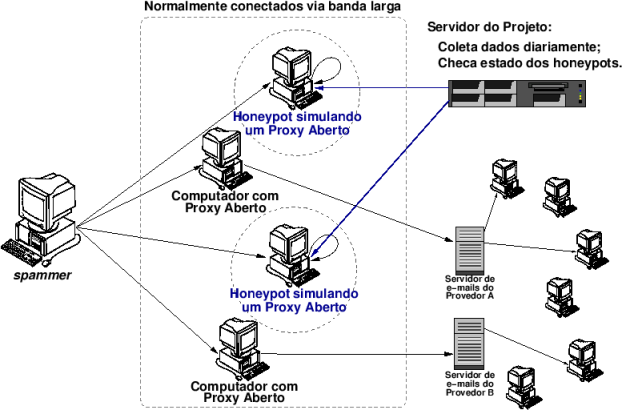
\includegraphics[scale=0.8]{img/honeypot.png} \\
        {\small Fonte: CERT (2007).} 
    \end{figure}
    
    Apesar de o Gráfico \ref{fig:plot_blacklist} apresentar subidas e descidas acentudas na contagem dos IPs listados na \textit{blacklist}, não foi evidenciada nenhuma relação imediata entre a quantidade de IPs listados com as tratativas implementadas em firewall para tentar mitigar o problema, o que caracteriza que o \textit{spam} está originando-se na rede interna dos assinantes e trafegando na internet pela camada de aplicação, como pode ser visto no relatório apresentado no Anexo A, que relata a detecção através de tráfego HTTP. 
    
    A CBL oferece a opção de remoção manual de um IP listado, porém essa ação não soluciona o problema de fato, uma vez que caso a infecção persista, muito provavelmente o IP retornará à listagem. Por isso, a melhor solução para o problema da \textit{blacklist} é a correção efetiva de vulnerabilidades existentes na rede, sendo que após um período de 28 dias sem nenhuma ocorrência, automaticamente o IP é removido da lista.

\section{Vulnerabilidades de rede}

    O CERT.br (Centro de Estudos, Resposta e Tratamento de Incidentes de Seguranca no Brasil) é responsável por tratar incidentes de seguranca computacional envolvendo redes conectadas à internet brasileira. Por isso, possui rotina de analisar, por amostragem, IPs registrados pelo Registro.br e notificar os responsáveis pelo AS no qual foi detectada alguma vulnerabilidade.
    
    Vulnerabilidades de rede são exploradas através de portas abertas em dispositivos, um vez que é pela camada de transporte que é possível estabelecer conexão e enviar pacotes pela rede. Portas abertas de serviços mal configurados são fonte para ataques de invasão, envio de \textit{spam} e DDoS (negação de serviço).
    
    Dessa forma, o CERT.br faz, regularmente, amostragem de IPs dos ASs brasileiros para realizar varredura de portas abertas, filtrando portas de serviços específicos que possam ser explorados por atacantes na internet e notificando as operadoras responsáveis. Uma varredura de portas, ou \textit{scan} de portas, pode ser feita a partir de terminal de comando pela ferramenta {\tt nmap}. Através do comando Figura \ref{fig:nmap}, pode ser feita a verredura de todas as portas do \textit{host} 192.0.2.99, por exemplo.

    \begin{figure}[!htb]
        \centering
        \caption{Exemplo de uso do nmap para varredura completa de portas.} 
        \label{fig:nmap} 
        
        \begin{Verbatim}[fontsize=\normalsize]
            nmap -sU -sT -p- 192.0.2.99 -T5
        \end{Verbatim} 
        
        {\small Fonte: do autor (2020).} 
    \end{figure}
    
    Quando portas de serviços vulneráveis são detectadas como abertas, o CERT.br envia um e-mail contendo relatório detalhado da vulnerabilidade ao responsável pela administração daquele IP escaneado, além de forncer sugestões para correção do problema. O Anexo B é um e-mail enviado pelo CERT.br à Minasnet após detectar vulnerabilidade no protocolo SOCKS em dispositivos MikroTik na rede.
    
    As vulnerabilidades surgem devido a configuração errônea de CPEs por parte dos instaladores nas residências ou comércios, ou por parte dos analistas no núcleo da rede. A correção dessas vulnerabilidades pode ser resolvida com a configuração correta de todos os equipamentos, difícil de ser atingido devido ao fator humano ser responsável pela garantia das configurações. Assim, a melhor tratativa necessita ter a menor dependência com humanos, sendo neste trabalho utilizada abordagem de firewall para filtragem de portas e VPN para controlar o acesso. 
    
    As principais vulnerabilidades exploradas por atacantes que foram tratadas através do firewall implementado são as vulnerabilidades por obtenção de informações, por invasão e por negação de serviço, que geralmente estão nas notificações do CERT.br por serem recorrentes, quando identificadas.

\section{Implantação de VPN}

    A abordagem do trabalho é primeiro filtrar o acesso implementando um serviço de VPN e depois fazer a filtragem de portas. Para isso, foi adotado o OpenVPN\footnote{OpenVPN \url{https://openvpn.net} é uma VPN SSL open source.}, uma solução gratuita, customizável e portável para várias plataformas. OpenVPN é um serviço completo de VPN SSL que é executável em um servidor Linux, podendo integrá-lo com vários outros serviços e protolocos como for desejável. VPNs L2TP/IPSec e PPTP não possuem tanto recursos e flexibilidade como o OpenVPN suporta. Além disso, OpenVPN é um projeto open source, que conta com grande comunidade, com documentação e com fórum de suporte e de discussão. OpenVPN também possui serviços prontos para empresas e para usuários finais, com valor pago de assinatura pelos mesmos.
    
    O projeto da VPN é bem simples, possuindo apenas dois requisitos: deve ser instalada em um servidor único e possuir autenticação de dois fatores (2FA). Assim, o \textit{deploy} do servidor foi feito em uma VPS Debian Linux, mantida no datacenter da Minasnet, com as seguintes configurações de hardware compartilhadas, pois foi alocada uma máquina virtual para ser o servidor:
    
    \begin{enumerate}[label=\alph*)]
        \item processador: Intel Xeon X7550;
        \item quantidade de núcleos: 2;
        \item memória RAM: 2GB;
        \item disco: 60GB;
        \item capacidade de rede: 1Gbps;
    \end{enumerate}
    
    A configuração do servidor foi feita inicialmente aplicando uma camada básica de segurança, seguindo o princípio do privilégio mínimo, deixando somente as portas necessárias abertas e restringindo o acesso SSH somente ao usuário administrador. Foi elaborado manual desse procedimento inicial e está disponível para consulta no Apêndice B.
    
    Após aplicado o princípio do privilégio mínimo ao servidor base onde será implantada a VPN, foi feita toda a instalação e configuração do serviço OpenVPN, também sendo criado manual de todos as configurações efetuadas. O manual completo da implantação do servidor OpenVPN está disponível no Apêndice C.
    
\subsection{Configuração do serviço OpenVPN}
    
    A configuração do servidor OpenVPN consiste em criar uma infraestrutura de chave privada (PKI) utilizando da ferramenta de CLI EasyRSA\footnote{EasyRSA \url{https://github.com/OpenVPN/easy-rsa} é um utilitário de CA (\textit{Certification Authority}).}, responsável pela autoridade dos certificados SSL utilizados na VPN. É recomendado manter os servidores de PKI e de VPN em máquinas distintas (serviço de autenticação e de conexão separados), entretanto para a finalidade deste trabalho foi mantido um servidor monolítico.
    
    Com a PKI operacional, são feitas as configurações do OpenVPN propriamente ditas, sendo ajustado os parâmetros para funcionamento básico do serviço conforme desejado: permitir que usuários autentiquem-se via internet e acessem a intranet através do túnel criado por essa conexão.
    
    O sistema 2FA utiliza o certificado SSL (mantido pela PKI) e autenticação por usuário e senha (suportada pelo \textit{plugin} PAM do Linux). A vantagem em utilizar PAM é a simplicidade de manutenção das contas de usuários, que é feita utilizando {\tt adduser} para criar um novo usuário, {\tt passwd} para alteração da senha e {\tt deluser} para remoção do usuário do sistema.
    
    Além disso, foi criado um \textit{script} feito em Python para facilitar a criação de chaves e de usuários, ao invés de fazer manualmente os comandos do EasyRSA todas as vezes que for criar novos usuários. O o programa não consiste em uma aplicação CLI totalmente funcional, apenas é um \textit{script} para facilitar a chamada dos comandos de maneira automática, sendo que em caso de problemas, é demandado experiência em terminal de comando Linux para lidar com erros no EasyRSA, nas contas de usuários ou no gerenciador de serviços {\tt systemd}. É possível construir uma interface mais robusta para gestão da VPN, web por exemplo, porém está fora do escopo deste trabalho.
    
    Além do servidor OpenVPN de produção, também é mantido um servidor OpenVPN de homologação, que está instalado em outra VPS com PKI distinta, com a finalidade de efetuar testes de funcionalidades sem afetar o ambiente em produção.
    
    O ambiente em produção mantém conexão de dezenas de usuários simultaneamente sem perca de desempenho, servindo de porta de entrada à rede privada do provedor. A configuração atual permite que somente seja possível acessar equipamentos de núcleo da rede através da VPN, restringindo e controlando o acesso remoto a equipamentos críticos somente a usuários autorizados, minimizando a probabilidade de incidência de ataques de invasão nos mesmos.
    
    O servidor OpenVPN principal está na rotina de backup automático dos servidores do datacenter da Minasnet, isso garante tolerância a falhas caso o servidor em produção seja corrompido, sendo somente necessário restauração de uma imagem do servidor que não seja perdido nenhum certificado da PKI, deste que o \textit{check-point} esteja em um instante após inserções de um novo usuário. Como a frequência do backup é semanal e não são adicionados novos usuários com tanta frequência, os impactos após uma inconsistência no servidor tendem a ser mínimos.
    
\subsection{Considerações sobre o servidor OpenVPN}

    A manutenção de um servidor OpenVPN demanda perícia em ambiente Linux, pois resolução de falhas requer análise de log do {\tt systemd}. Um detalhe é que o serviço da VPN não se inicia automaticamente quando o servidor é reiniciado, devido a necessidade de inserção manual do \textit{passphrase} da PKI em prompt no terminal de comandos.
    
    Outro detalhe é que os certificados SSL têm prazo de validade de 3 anos, sendo que não é possível renová-los para estender a data de validade. É importante monitorar a validade dos certificados e gerar novos depois de vencidos para que não haja transtorno para os usuários da VPN.
    
\section{Implementação de firewall}

    Com a VPN operacional, o próximo passo para implementação de segurança na rede é a configuração do sistema de firewall para filtragem de pacotes suspeitos. A finalidade do firewall é mitigar as vulnerabilidades elencadas pelas notificações do CERT.br, bem como garantir a aplicação das políticas de segurança de rede adotadas pelo ISP.
    
    A abordagem de firewall deste trabalho é simples e eficiente, fazendo filtragem por endereços IP e por números de porta, ou seja, o firewall vai inspecionar os cabeçalhos dos pacotes nas camadas de rede e de transporte. Existem modelos de firewall que inspecionam pacotes na camada de aplicação (firewall \textit{layer} 7), porém requerem muito poder de processamento e podem afetar negativamente o \textit{throughput} da rede, sendo dedicados às redes corporativas (universidades e grandes corporações) ao invés de provedores de internet. Filtrar IP e porta é o suficiente para a função do ISP.
    
    Antes da implantação deste trabalho, não existia firewall na rede de acesso dos clientes da Minasnet, ou seja, todos os CPEs dos clientes estavam expostos à internet sem nenhum filtro, sendo a única camada de segurança a manutenção de senhas fortes nos equipamentos e configuração correta por parte dos instaladores, algo que nem sempre ocorria. Houve relatos, por exemplo, de antenas Ubiquiti e MikroTik que foram infectadas por \textit{worms} devido às vulnerabilidades nas quais os equipamentos estavam expostos.
    
    Após elencadas as vulnerabilidades nas quais os equipamentos da rede são suscetíveis, a tarefa é implementar as regras de firewall para colocá-las em produção em um dispositivo que faça interface entre os tráfegos de rede, ou seja, que fique intermediando o caminho por onde passarão todos os pacotes. A abordagem deste trabalho utiliza do firewall nativo da plataforma RouterOS dos roteadores MikroTik, que possui seu funcionamento básico semelhante ao iptables do Linux, pois a próprioa plataforma é construída sobre o \textit{kernel} Linux.
    
    Os requisitos de firewall desenvolvidos para a Minasnet, inicialmente, são os seguintes: 
    
    \begin{enumerate}[label=\alph*)]
        \item negar o acesso remoto aos equipamentos primários dos clientes, que desempenham a função de cliente PPPoE;
        \item permitir somente que o NOC e o Help Desk acessem remotamente os equipamentos dos clientes;
        \item permitir que clientes de IP fixo fiquem expostos à internet, sem filtragem por firewall;
        \item negar que clientes acessem a intranet do ISP;
        \item aplicar filtros que corrijam vulnerabilidades detectadas na rede.
    \end{enumerate}
    
\subsection{Regras de firewall no RouterOS}

    O objetivo deste firewall é filtrar conexões de entrada que caracterizem como acesso ilegal a equipamentos, baseado em regras definidas por IP e porta. Filtrar consiste em descartar pacotes de acordo com as regras.
    
    A topologia utilizada para implantação do firewall aplica as regras diretamente ao concentrador, pois é nele que está a origem (ou destino, dependendo do ponto de vista) do tráfego dos clientes. Colocar outro equipamento intermediando o concentrador com finalidade de firewall não é suficiente, pois não é possível filtrar conexões entre clientes de um mesmo concentrador de acordo com a metodologia utilizada neste trabalho, isso porque a comutação de pacotes é feita em memória neste caso.
    
    De acordo com a documentação do RouterOS \cite{fwmikrotik}, para implementar o firewall de acordo com os requisitos supracitados, são utilizados os seguintes parâmetros oferecidos na tabela \textit{filter} do firewall:
    
    \begin{enumerate}[label=\alph*)]
        \item {\tt address-list}: estrutura de dados do tipo lista contendo endereços que serão alvo das regras, para auxiliar na construção fracamente acoplada dos componentes do firewall;
        \item {\tt action}: ação que o firewall deve executar quando a regra for acionada, como o objetivo é filtrar, será utilizada como ação \textit{drop};
        \item {\tt chain}: caminho que o pacote faz no roteador, como os pacotes que serão filtrados estão sendo roteados, utiliza-se da cadeia \textit{forward};
        \item {\tt protocol}: protocolo de transporte, sendo TCP ou UDP;
        \item {\tt in-interface} ou {\tt out-interface}: interface alvos das regras, sendo neste caso todos os clientes PPPoE;
        \item {\tt src-port} ou {\tt dst-port}: número de porta que serão filtradas pelo firewall.
    \end{enumerate}

    A construção das regras de firewall foram feitas através de \textit{script} nativo para a plataforma. A seguir estão exemplos da implementação de algumas regras básicas que atendem aos requisitos definidos anteriormente, sendo que na Figura \ref{fig:firewall_addrlist} está codificada a primeira etapa da construção do firewall: a definição das listas de IP nas quais as regras de filtragem serão trabalhadas, sendo elas as redes de gerência, que têm acesso privilegiado em toda a rede do ISP, a rede de clientes que contrataram o serviço de IP fixo e desejam ficar expostos à internet, e a rede de Bogons, que neste caso são endereços privados do ISP e não devem ser acessíveis pelos assinantes.
    
    A utilização de listas de IP não é obrigatória para configuração das regras de firewall, sendo possível inserir cada um dos IPs diretamente. O problema é que a manutenabilidade do firewall fica prejudicada, assim as listas deixam os componentes fracamente conectados e permite que qualquer alteração de IP não necessite de alteração nas regras propriamente ditas, além de deixar o código mais legível, sendo assim uma boa prática no desenvolvimento do firewall.
    
    \begin{figure}[!htb]
        \centering
        \caption{Exemplo de criação de address-list para o firewall do RouterOS.} 
        \label{fig:firewall_addrlist}
        
        \begin{Verbatim}[fontsize=\normalsize]
            /ip firewall address-list
            add comment="IP FIXO CLIENTES"                  \
                address=203.0.113.128/25 list=rede_ip_fixo
            add comment="SERVIDOR VPN"                      \
                address=203.0.113.123 list=rede_gerencia
            add comment="HELP DESK"                         \
                address=203.0.113.124 list=rede_gerencia
            add comment="ESCRITORIO NOC"                    \
                address=203.0.113.125 list=rede_gerencia
            add comment="BOGONS"                            \
                address=10.0.0.0/8 list=rede_privada
            add comment="BOGONS"                            \
                address=172.16.0.0/12 list=rede_privada
            add comment="BOGONS"                            \
                address=192.168.0.0/16 list=rede_privada
        \end{Verbatim} 

        {\small Fonte: do autor (2020).} 
    \end{figure}
    
    Um dos primeiros requisitos citados para implementação firewall foi a necessiadade de impedir a invasão aos equipamentos de clientes, sendo possibilitado o acesso somente às redes gerenciais da empresa (NOC e Help Desk). Assim, na Figura \ref{fig:drop_cpe} é feito o bloqueio de todo acesso externo nas portas de gerência em todos os assinantes, exceto IP fixo, a fim de garantir o cumprimento do requisito de segurança.
    
    \begin{figure}[!htb]
        \centering
        \caption{Regra de firewall para controle de acesso aos CPEs.} 
        \label{fig:drop_cpe}
        
        \begin{Verbatim}[fontsize=\normalsize]
            /ip firewall filter
            add comment="DROP GERENCIA DE CPE"  \
                action=drop                     \
                chain=forward                   \
                out-interface=all-ppp           \
                src-address-list=!rede_gerencia \
                dst-address-list=!rede_ip_fixo  \
                dst-port=0-1023                 \
                protocol=tcp
        \end{Verbatim} 

        {\small Fonte: do autor (2020).} 
    \end{figure}
    
    Outro requisito está codificado na Figura \ref{fig:drop_bogon}, que impede a descoberta e o acesso às redes bogons, que são IPs privados muitas vezes utilizados para endereçar roteadores e servidores do núcleo da rede, sendo necessário bloquear toda conexão de saída em todos os clientes com destino para lista de redes privadas, a fim de garantir o princípio do privilégio mínimo a esses equipamentos, que devem ser acessíveis somente à equipe do NOC por se tratar de dispositivos que operam a parte crítica da rede. Assim, um hacker que conseguir elencar e explorar alguma vulnerabilidade nesses equipamentos, pode causar um prejuízo enorme ao ISP.
    
    \begin{figure}[!htb]
        \centering
        \caption{Regra de firewall para bloqueio de acesso à rede privada do provedor.} 
        \label{fig:drop_bogon}
        
        \begin{Verbatim}[fontsize=\normalsize]
            /ip firewall filter
            add comment="DROP REDE BOGON"     \
                action=drop                   \
                chain=forward                 \
                in-interface=all-ppp          \
                dst-address-list=rede_privada
        \end{Verbatim} 

        {\small Fonte: do autor (2020).} 
    \end{figure}
    
    A Figura \ref{fig:drop_socks} tem a implementação do filtro que impede ataque de \textit{spam} a partir de servidores SOCKS abertos em Mikrotik, bloqueando toda conexão de entrada na porta 4145 TCP em todos os assinantes, sem exceção, por razões de segurança, uma vez que a notificação do CERT.br disponível no Anexo B relata que inclusive clientes de IP fixo estão vulneráveis. Como essa regra foi desenvolvida com a finalidade de corrigir o problema citado no e-mail, todos os assinantes são alvo dessa filtragem.
    
    \begin{figure}[!htb]
        \centering
        \caption{Regra de firewall para correção da vulnerabilidade por SOCKS notificada pelo CERT.br.} 
        \label{fig:drop_socks}
        
        \begin{Verbatim}[fontsize=\normalsize]
            /ip firewall filter
            add comment="DROP SOCKS 4145" \
                action=drop               \
                chain=forward             \
                out-interface=all-ppp     \
                dst-port=4145             \
                protocol=tcp
        \end{Verbatim} 

        {\small Fonte: do autor (2020).} 
    \end{figure}
    
    Não será exposto o script completo de configuração do firewall dos concentradores da Minasnet neste documento, por questão de segurança e de confidencialidade, uma vez que pessoas mal intencionadas poderiam explorar alguma vulnerabilidade que tenha passada despercebida na metodologia utilizada. Mesmo que não exista sistema 100\% seguro, mantendo confidencialidade é possível dificultar o trabalho dos atacantes. Por isso, ficaram descritos aqui somente esses exemplos.
    
\subsection{Considerações sobre o firewall}
    
    A criação de regras de firewall é uma tarefa simples quando se conhece os recursos da plataforma na qual está trabalhando, porém requer cautela, pois configuração errônea pode comprometer a navegação dos assinantes ou então aferar negativamente o processamento dos roteadores nos quais foram feitos a implantação das regras. Devido a familiaridade com iptables, o firewall do RouterOS é intuitivo para quem tem experiência com o sistem Linux.
    
    Após colocar o firewall da Minasnet em produção, notificações recorrentes do CERT.br cessaram, no entanto novas vulnerabilidades são elencadas frequentemente pelos \textit{scanners} do grupo, surgindo a tarefa contínua a criação, a melhoria e o aperfeiçoamento das regras do firewall dos concentradores.
    
    A implantação de firewall no concentrador requer cuidado, uma vez que pode comprometer o desempenho da Routerboard. Por isso, foi feito monitoramento de consumo de CPU em diferentes horários do dia, inclusive em horários de pico por volta das 20h, para constatar que o firewall desenvolvido não afetou o desempenho do roteador consideravelmente, sendo que o processamento do concentrador já era concorrido pela manutenção das \textit{queues} e do CGNAT.
    
    A dificuldade em implantar regras de firewall é o risco de afetar a navegação no ambiente em produção, sendo necessário ambiente de testes antes de ser feito o \textit{deploy}. Na Minasnet, foram utilizadas de conjuntos de RB750 e pequenos servidores web instalados no computador para testar a filtragem dos pacotes antes de colocar em operação. Também é possível fazer os testes através de simuladores, como o GNS3, no qual é possível construir um ambiente de homologação completo para redes e sistemas distribuídos.
    
  \chapter{CONCLUSÃO}

    No curso de Bacharelado em Ciência da Computação da Universidade Federal de Lavras, o estudante tem a oportunidade de aprender os aspectos teóricos que fundamentam as vastas tecnologias digitais que são indispensáveis à sociedade contemporânea, as Tecnologias da Informação e Comunicação (TICs). Dentro das TICs, destaca-se uma das maiores e mais poderosas ferramentas desenvolvida pelo ser humano: a internet, que foi o destaque neste trabalho.

    O trabalho serviu como ponte entre o conhecimento acadêmico e o conhecimento prático. Cálculos de sub-redes podiam até parecer não ter sentido em listas de exercícios em disciplina da graduação, mas com os cálculos de endereçamento e de implantação de CGNAT mostraram sua importância para garantir que a camada lógica da internet funcione e permita que os assinantes naveguem pela rede. Não somente isso, adotar práticas e políticas de segurança com adoção de firewall e VPN também possibilitou a aplicação dos princípios que antes foram abordados somente em laboratório e em estudos de caso fictícios.
    
    O legado gerencial deixado pelo estágio está no monitoramento contínuo dos serviços como estratégia de inteligência de negócios na empresa, pois é através dele que é possível reagir às falhas o quanto antes, bem como prever problemas de antemão, a fim de garantir a qualidade do serviços prestado a população. O trabalho abordou a parte mais técnica de operação de redes, mas o dia a dia gira em torno da gestão e do monitoramento de incidentes.
    
    Os objetivos foram alcançados sem muitas dificuldades operacionais para a execução dos mesmos, pois o estagiário já havia uma bagagem teórica consolidada e o trabalho serviu como meio para praticar o conhecimento e gerar valor. As dificuldades foram recorrentes devido à insegurança em aplicar alterações em sistemas em produção com milhares de clientes navegando, algo normal quando se pensa que uma falha pode "parar tudo" em questão de segundos.

    Apesar de na universidade existirem atividades e projetos em que o estudante possa obter conhecimento prático dos tópicos abordados em sala de aula, através de trabalhos práticos em laboratórios ou simuladores, de projetos de extensão acadêmica ou mesmo em empresas juniores, o estudante não conseguirá uma visão ampla da dimensão do assunto, por estar lidando com casos particulares e restritos. Por isso é importante a realização do estágio em uma organização, onde se pode aprender e desenvolver habilidades práticas em um ambiente em produção e que presta serviço a toda a comunidade, seja em nível local, regional, nacional ou internacional.
    
    Por isso a realização deste trabalho de estágio supervisionado na organização Minasnet foi importante para a maturação do estudante como profissional da área de redes, pois foi o momento quando se colocou em prática os protocolos aprendidos na disciplina de Redes de Computadores como também as arquiteturas de sistemas distribuídos, em nível de infraestrutura, vistos na disciplina de Arquitetura de Computadores e em Sistemas Distribuídos. De fato, o estágio obordou assuntos que foram além dessas disciplinas básicas da área de infraestrutura, o que demonstra uma falta de disciplinas ofertadas na mesma área por parte do Departamento de Ciência da Computação. Durante o curso, foram mínimas (se não inexistentes) disciplinas eletivas sobre assuntos de redes, o que está deixando o curso de Ciência da Computação focado quase que exclusivamente na camada de aplicação do Modelo OSI, com foco em desenvolvimento de aplicações. Não se pode deixar de lado a infraestrutura dos sistemas de computação e de informação, pois é ela que sustenta todas as aplicação que estão em operação na web hoje, por exemplo.
    

  % ==============================================================================
  % Incluindo bibliografia
  % \bibliographystyle{plain}         % estilo para labels em numeros
  % \bibliographystyle{alpha}         % estilo para labels em iniciais
  \bibliographystyle{abntex2-alf}     % estilo para referências usando ABNT, precisa instalar o abntex para usar!!!

  % inclui Referências Bibliográficas
  \referencias
  \bibliography{referencias}               % arquivo exemplo refbib.bib
  % ==============================================================================
  % Incluindo anexos numerados com letras maiusculas.
  \apendices
  \begin{center}
  \normalsize{\textbf{APÊNDICE A -- Documentação de leitura rápida do py-cgnat}}
\end{center}

\pagestyle{empty} % remover numeração

\begin{figure}
    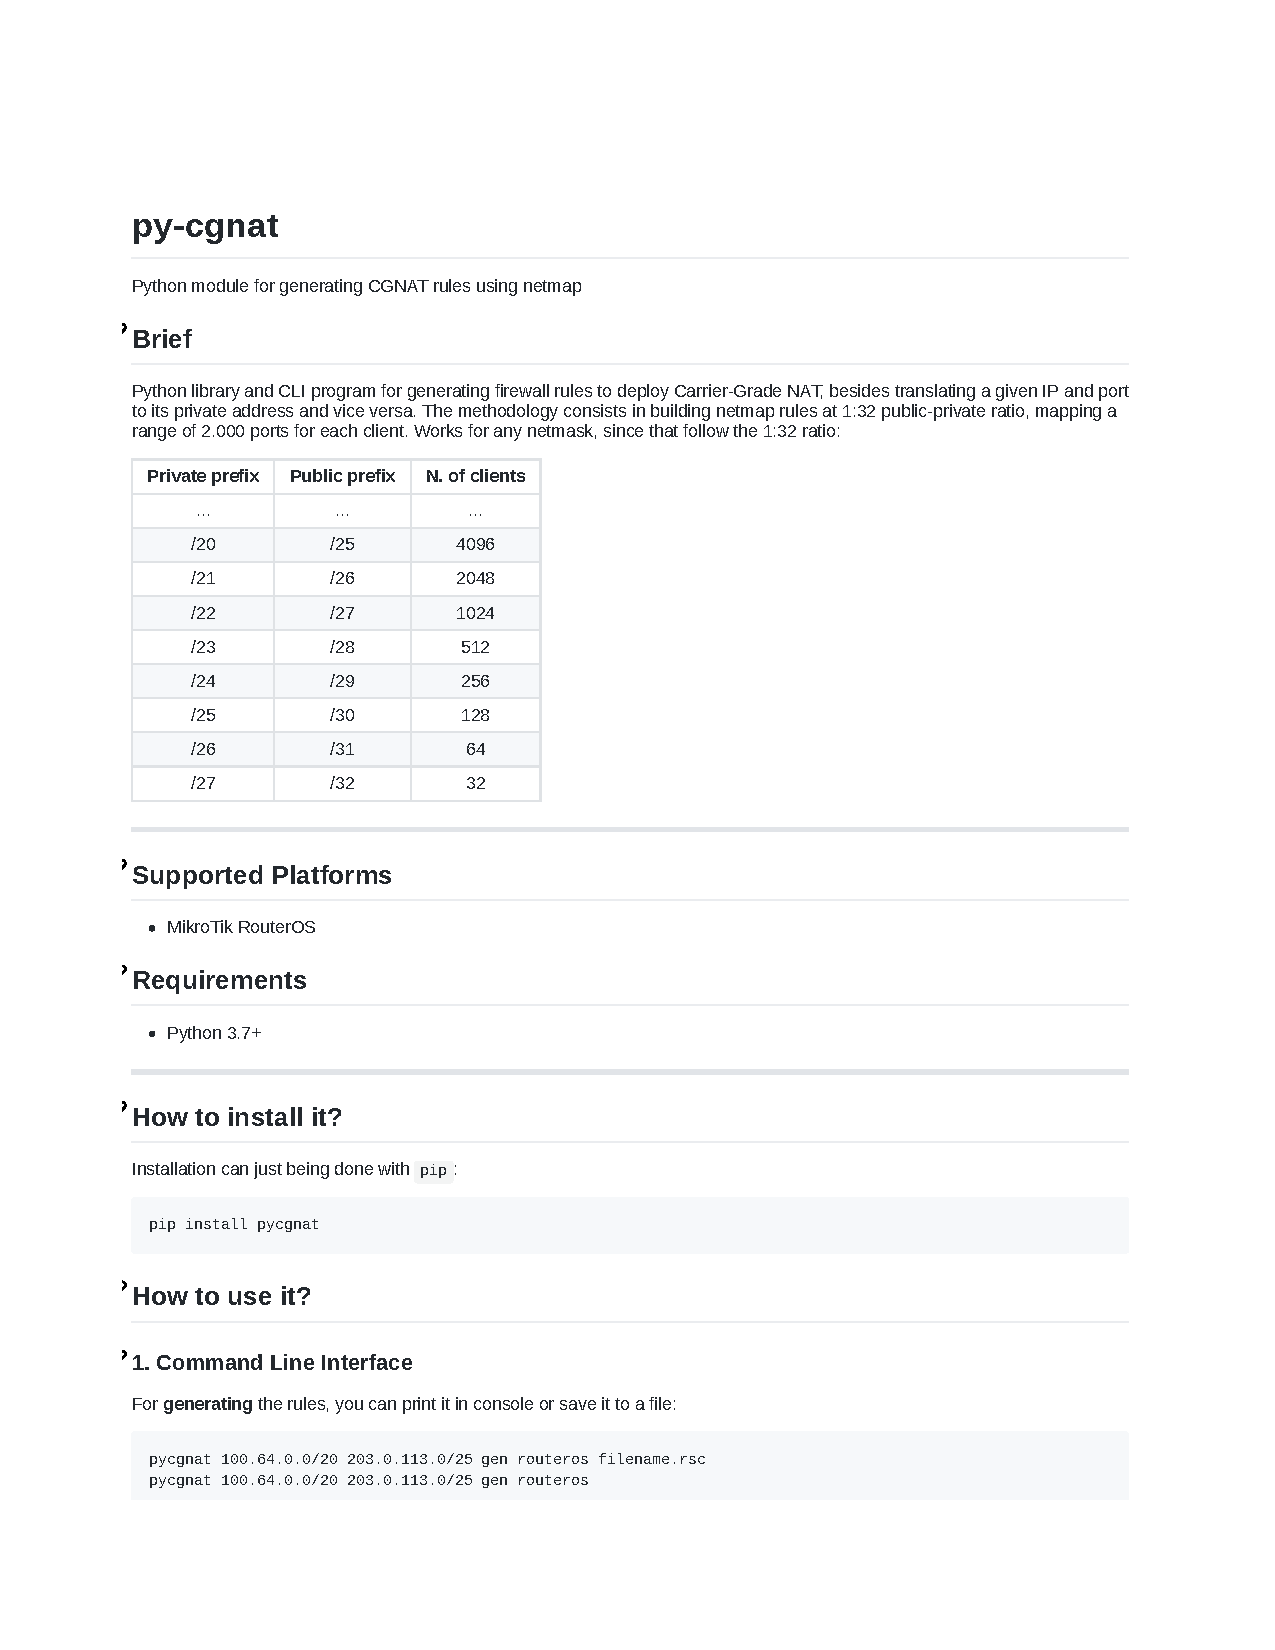
\includepdf[pages=1, offset=75 -75]{pdf/pycgnat-1.0b1-README.pdf}
\end{figure}

\newpage

\begin{figure}
    \includepdf[pages=2, offset=75 -75]{pdf/pycgnat-1.0b1-README.pdf}
\end{figure}
  \begin{center}
  \normalsize{\textbf{APÊNDICE B -- Manual para configuração básica de segurança em servidor Debian 9}}
\end{center}

\pagestyle{empty} % remover numeração

\begin{figure}
    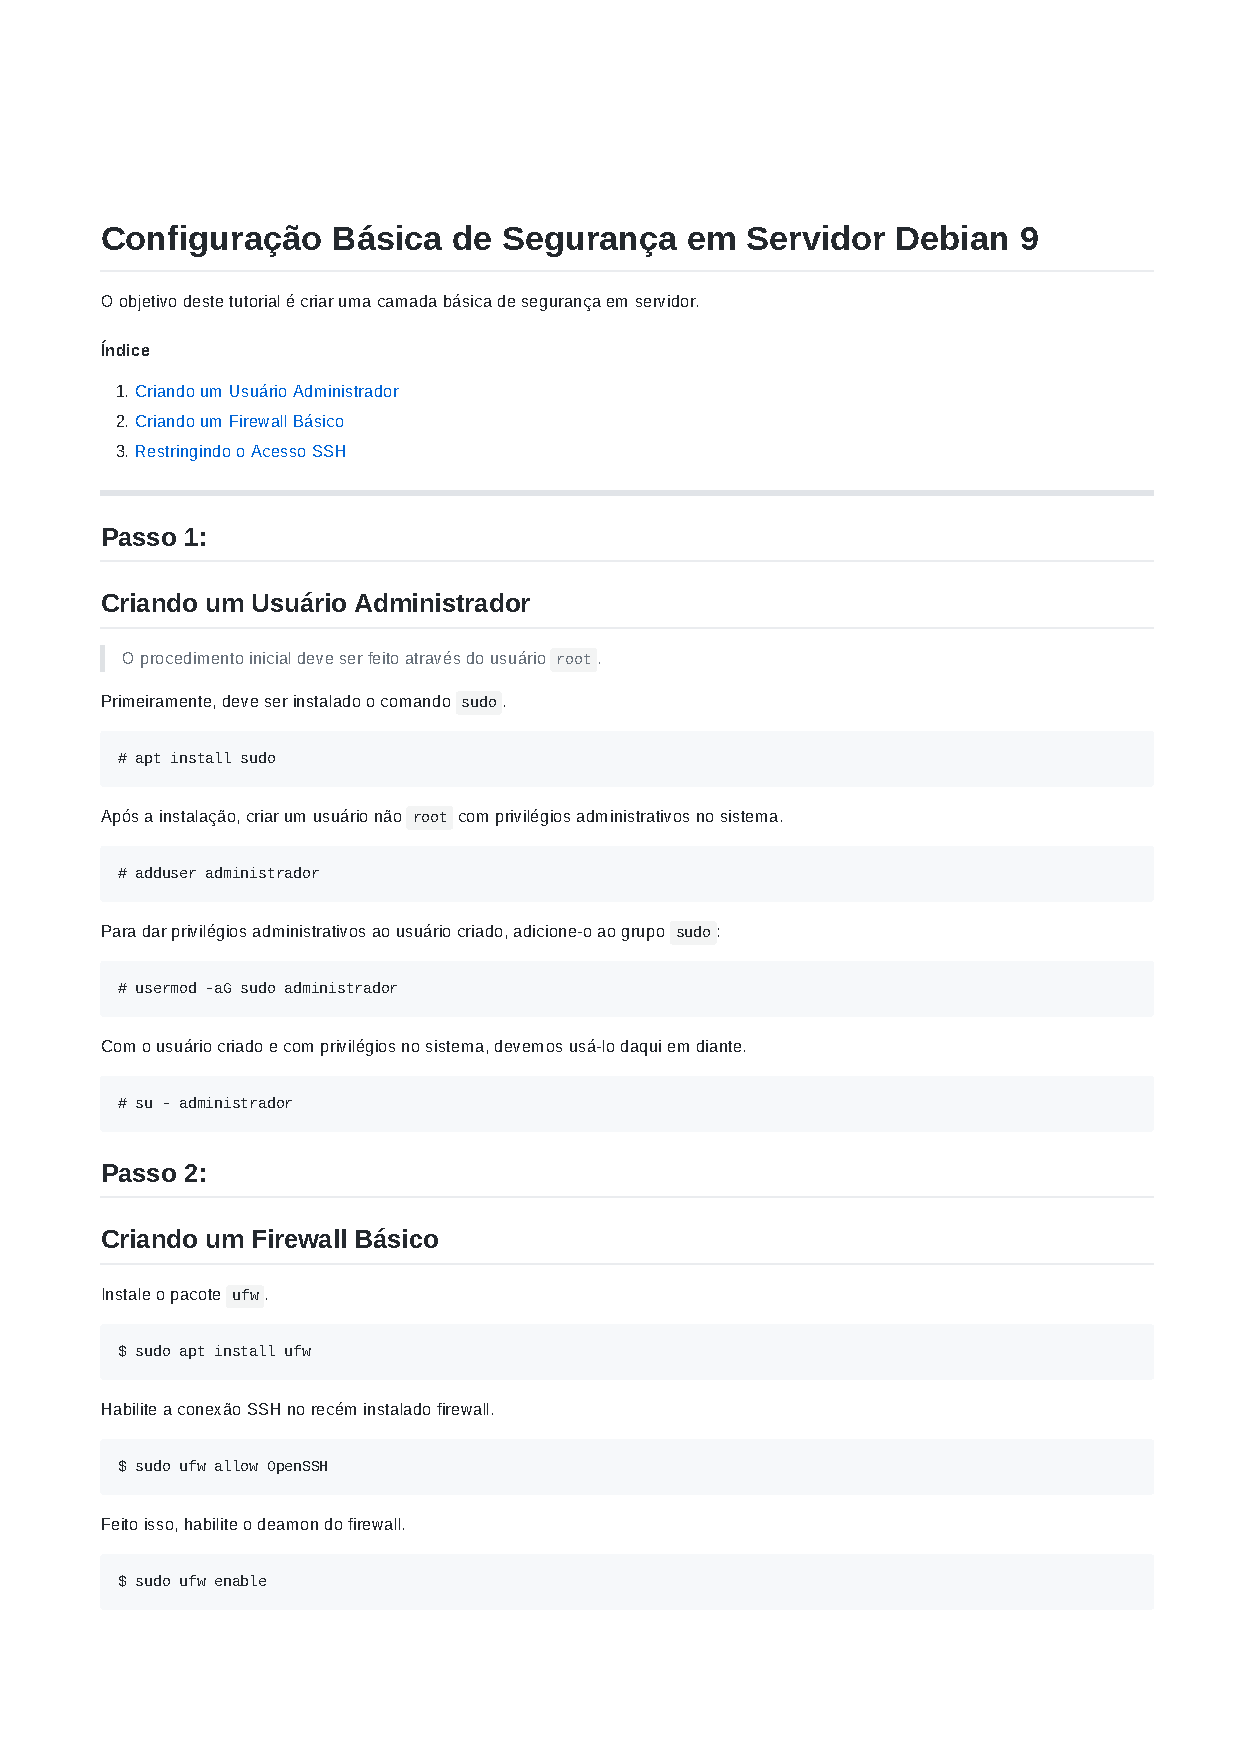
\includepdf[pages=1, offset=75 -75]{pdf/openvpn-server-base.pdf}
\end{figure}

\newpage

\begin{figure}
    \includepdf[pages=2, offset=75 -75]{pdf/openvpn-server-base.pdf}
\end{figure}

  \begin{center}
  \normalsize{\textbf{APÊNDICE C -- Manual para instalação de servidor OpenVPN no Debian 9}}
\end{center}

\pagestyle{empty} % remover numeração

\begin{figure}
    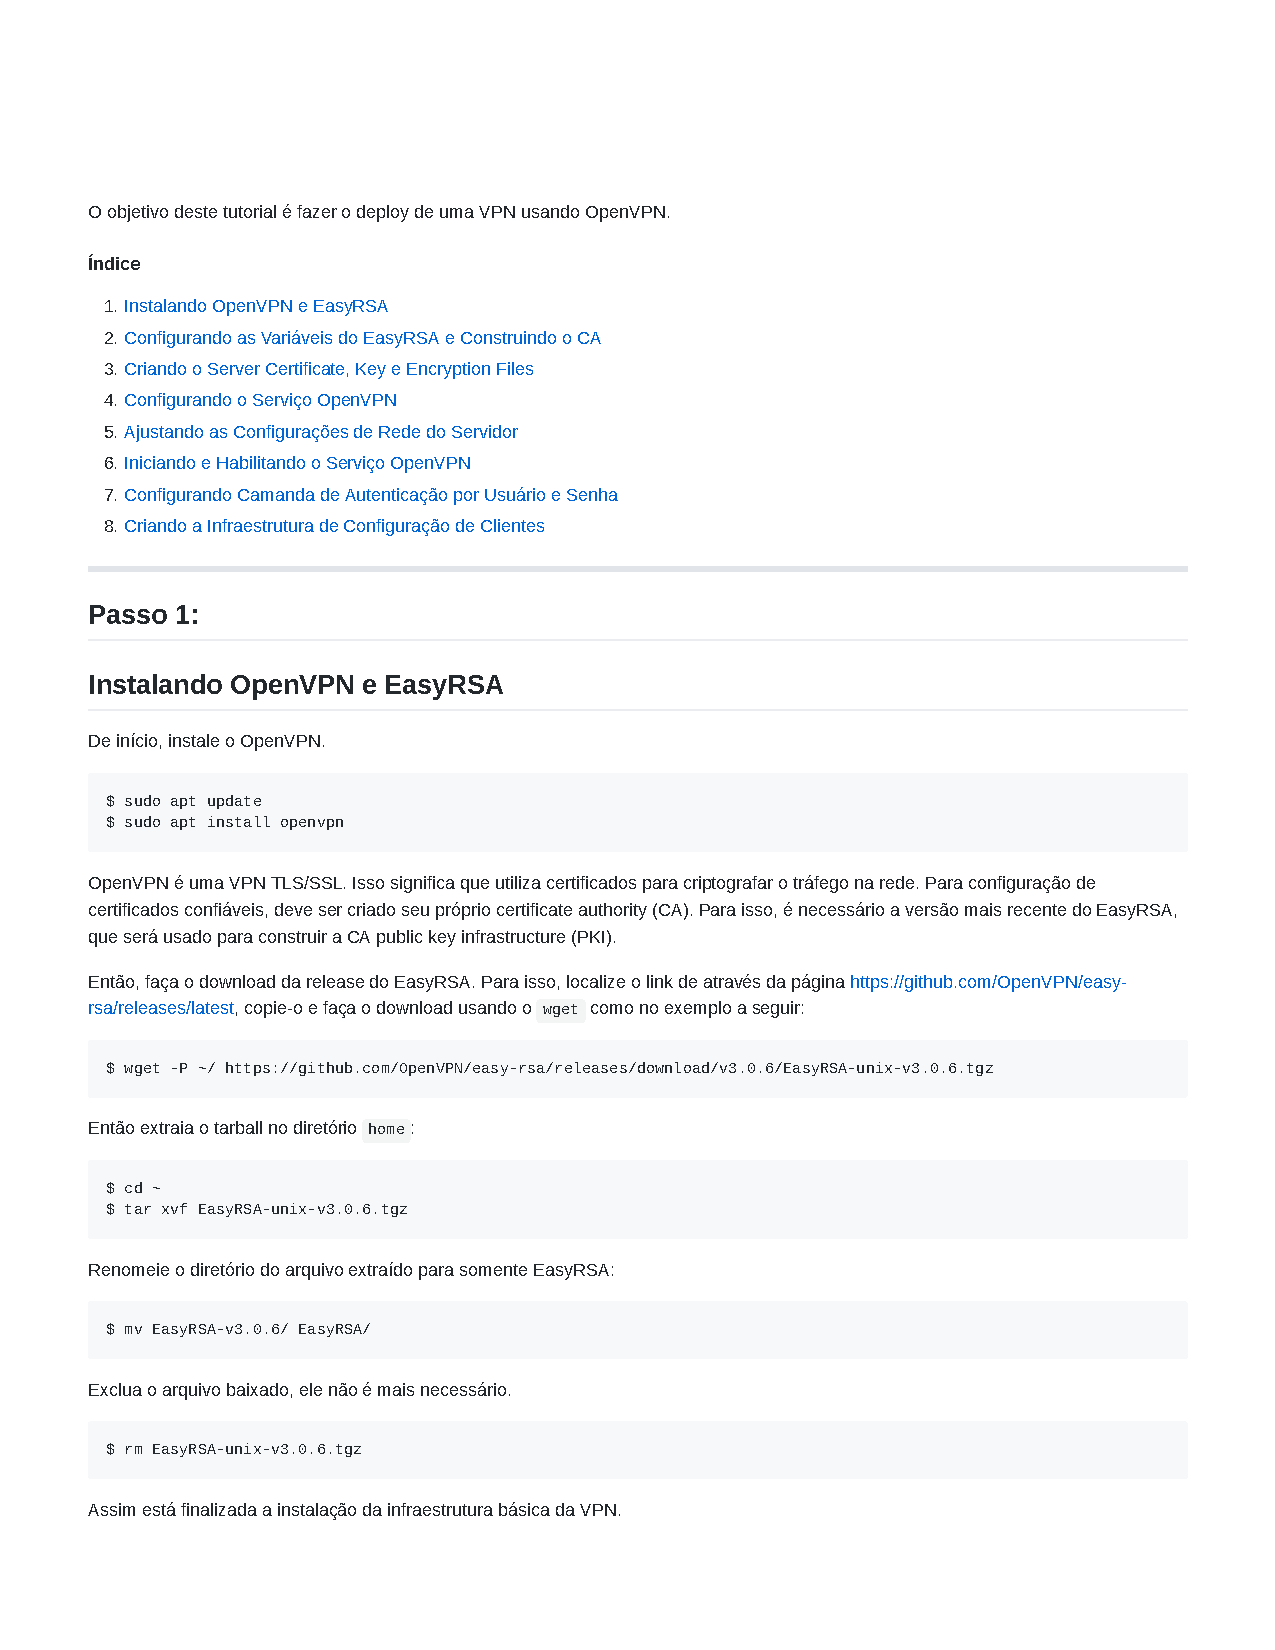
\includepdf[pages=1, offset=75 -75]{pdf/openvpn-deploy.pdf}
\end{figure}

\newpage

\begin{figure}
    \includepdf[pages=2, offset=75 -75]{pdf/openvpn-deploy.pdf}
\end{figure}

\newpage

\begin{figure}
    \includepdf[pages=3, offset=75 -75]{pdf/openvpn-deploy.pdf}
\end{figure}

\newpage

\begin{figure}
    \includepdf[pages=4, offset=75 -75]{pdf/openvpn-deploy.pdf}
\end{figure}

\newpage

\begin{figure}
    \includepdf[pages=5, offset=75 -75]{pdf/openvpn-deploy.pdf}
\end{figure}

\newpage

\begin{figure}
    \includepdf[pages=6, offset=75 -75]{pdf/openvpn-deploy.pdf}
\end{figure}

\newpage

\begin{figure}
    \includepdf[pages=7, offset=75 -75]{pdf/openvpn-deploy.pdf}
\end{figure}

\newpage

\begin{figure}
    \includepdf[pages=8, offset=75 -75]{pdf/openvpn-deploy.pdf}
\end{figure}
  \begin{center}
  \normalsize{\textbf{ANEXO A -- Um relatório justificando listagem de IP na blacklist CBL}}
  \label{relatorio_blacklist}
\end{center}

\pagestyle{empty} % remover numeração

\begin{figure}
    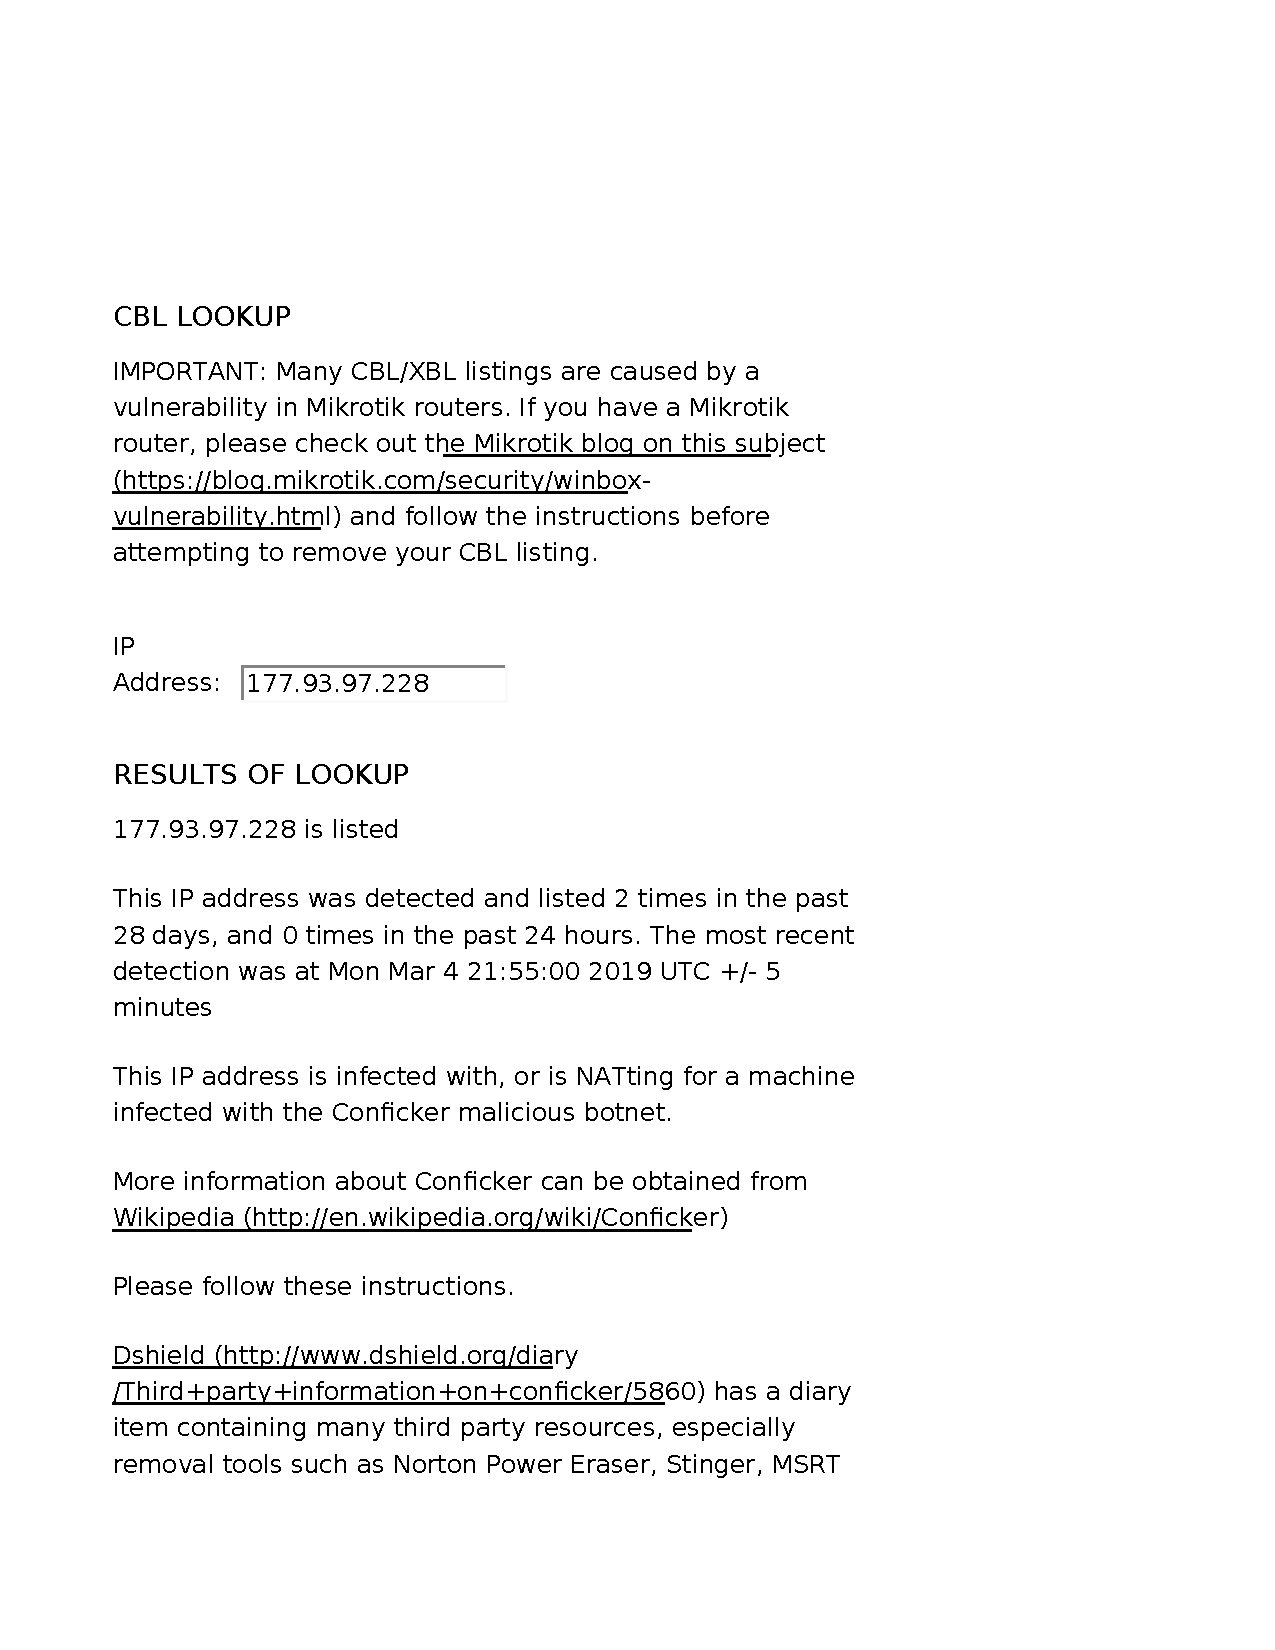
\includepdf[pages=1, offset=75 -75]{pdf/177-93-97-228-CBL.pdf}
\end{figure}

\newpage

\begin{figure}
    \includepdf[pages=2, offset=75 -75]{pdf/177-93-97-228-CBL.pdf}
\end{figure}

\newpage

\begin{figure}
    \includepdf[pages=3, offset=75 -75]{pdf/177-93-97-228-CBL.pdf}
\end{figure}

\newpage

\begin{figure}
    \includepdf[pages=4, offset=75 -75]{pdf/177-93-97-228-CBL.pdf}
\end{figure}

\newpage

\begin{figure}
    \includepdf[pages=5, offset=75 -75]{pdf/177-93-97-228-CBL.pdf}
\end{figure}

  \begin{center}
  \normalsize{\textbf{ANEXO B -- Um e-mail de alerta de segurança enviado pelo CERT.br}}
\end{center}

\pagestyle{empty} % remover numeração

\begin{verbatim}
From: "CERT.br" <cert@cert.br>
Subject: Alerta: [AS 262488] Mikrotik Possivelmente Comprometido - SOCKS 4145
Date: 3 June 2019 09:54:05 GMT-3
To: contato@minasnet.net
Cc: cert@cert.br
Reply-To: cert@cert.br

Caro responsável,

Os IPs no log ao final dessa mensagem possivelmente são de dispositivos
Mikrotik em sua rede que foram comprometidos e que estão sendo abusados
intensamente para o envio de spam.

Esse comprometimento habilita o serviço SOCKS na porta 4145/tcp
que pode ser abusado para diversas atividades, principalmente para o
envio de spam.

Essas atividades estão consumindo recursos de sua rede e provavelmente
incluindo seus IPs em listas de bloqueio.

Se você não for a pessoa correta para corrigir este problema, por
favor repasse essa mensagem para alguém da sua organização que possa
fazê-lo.

Gostaríamos de solicitar que:
1. cada dispositivo associado aos IPs abaixo fosse revisado e, se
  confirmada a suspeita de comprometimento, o problema seja resolvido
  (com a desativação do serviço SOCKS, alteração das senhas e atualização
   do RouterOS);
2. aumente-se o nível de monitoração da rede para determinar se outros
  dispositivos da sua rede também estão sofrendo do mesmo problema.

Sugestões de como realizar esses dois itens seguem abaixo.

* Como resolver o comprometimento dos dispositivos Mikrotik?
 1. Verifique a existência de um serviço SOCKS atendendo na
    porta 4145/tcp, executando o seguinte comando:
    /ip socks print
    Se o serviço estiver marcado como habilitado (enabled = yes),
    desabilite-o com o seguinte comando:
    /ip socks set enable=no
 2. Atualize a versão do Router OS para a última versão
    "Long-term/bugfix" ou "Stable/current", de acordo com as instruções
    do fabricante disponíveis na seguinte URL:
    https://wiki.mikrotik.com/wiki/Manual:Upgrading_RouterOS
 3. Apenas depois de atualizar o sistema altere a senha com o comando
    abaixo:
    /user set USUARIO password=NOVA_SENHA
    onde USUARIO é o usuário utilizado para conectar no mikrotik

* Como identificar outros dispositivos sendo abusados pela mesma
 técnica?
 Sugerimos também que monitore regularmente o tráfego de sua rede
 através do uso de netflow para identificar esse problema. Uma
 sugestão seria monitorar o tráfego na porta 4145/tcp e observar o
 aumento anormal de conexões com destino às portas 25/tcp e 587/tcp.

* O que é o CERT.br?
 O CERT.br -- Centro de Estudos, Resposta e Tratamento de Incidentes
 de Segurança no Brasil -- é o Grupo de Resposta a Incidentes de
 Segurança para a Internet brasileira, mantido pelo NIC.br do Comitê
 Gestor da Internet no Brasil.  É o grupo responsável por tratar
 incidentes de segurança em computadores, envolvendo redes conectadas
 à Internet brasileira.

 IP              | ASN    | Porta | Status | Timestamp            | Resultado do 
                                                                    Teste
=============================================================================
177.66.52.134    | 262488 |  4145 | OPEN   | 2019-06-03T08:50:01Z | SMTP banner: 
                                                                    confirmed
177.66.52.137    | 262488 |  4145 | OPEN   | 2019-05-27T18:02:30Z | SMTP banner: 
                                                                    confirmed
177.66.52.195    | 262488 |  4145 | OPEN   | 2019-05-28T20:55:06Z | SMTP banner: 
                                                                    confirmed
177.66.52.232    | 262488 |  4145 | OPEN   | 2019-05-28T20:55:17Z | SMTP banner: 
                                                                    confirmed
177.66.52.252    | 262488 |  4145 | OPEN   | 2019-05-29T22:44:48Z | SMTP banner: 
                                                                    confirmed
179.106.162.108  | 262488 |  4145 | OPEN   | 2019-05-27T23:52:08Z | SMTP banner: 
                                                                    confirmed
179.106.162.145  | 262488 |  4145 | OPEN   | 2019-05-27T18:04:40Z | SMTP banner: 
                                                                    confirmed
179.106.166.57   | 262488 |  4145 | OPEN   | 2019-05-30T14:10:38Z | SMTP banner: 
                                                                    confirmed
179.106.166.92   | 262488 |  4145 | OPEN   | 2019-05-27T18:04:41Z | SMTP banner: 
                                                                    confirmed
=============================================================================

Cordialmente,
--
CERT.br/NIC.br
<cert@cert.br>
https://www.cert.br/
\end{verbatim}

  % ==============================================================================
  % Fim do texto
\end{document}
